% !TEX encoding = UTF-8 Unicode
% !TEX root = DesignDocument.tex

\documentclass{book}

% !TEX root = DesignDocument.tex



\usepackage[width=6.5in, height=9.2in, top=1.0in, papersize={8.5in,11in}]{geometry}
\usepackage[pdftex]{graphicx}
\usepackage{amsmath}
\usepackage{amsthm}
\usepackage{amssymb}
%\usepackage{txfonts}
\usepackage{textcomp}
\usepackage{amsthm}

\usepackage[all]{xy}
\usepackage{fancyhdr}
\pagestyle{fancy}
\usepackage{hyperref}
\usepackage{verbatim}
\usepackage{algorithm}
\usepackage{algorithmic}
\usepackage{array}
\usepackage{color}
\usepackage{listings}
\usepackage{calc}
\usepackage{doxygen}
\usepackage[utf8]{inputenc}
\usepackage{makeidx}
\usepackage{multicol}
\usepackage{multirow}
\usepackage[table]{xcolor}
\usepackage{tabularx}
\usepackage{framed}
\usepackage{xspace}
\usepackage{etex}
\usepackage{todonotes}
\usepackage{pdfpages}
\usepackage{pgfgantt}


%% Computer Modern Bright Font
%\usepackage{cmbright}
%\usepackage[T1]{fontenc}

%% Sans Serif Modern Font - similar to  Helvetica
\usepackage{lmodern}
\renewcommand*\familydefault{\sfdefault} %% Only if the base font of the document is to be sans serif
\usepackage[T1]{fontenc}


\definecolor{SDColor1}{rgb}{0,0,0}
\definecolor{SDColor2}{rgb}{0,0,0}
\definecolor{SDColor3}{rgb}{0,0,0}
\definecolor{SDColor4}{rgb}{0,0,0}
\definecolor{SDColor5}{rgb}{0,0,0}

%%%  --- Here are some other colors.  Keep it conservative --- %%%

%% Blue font color scheme
%\definecolor{SDColor1}{rgb}{.204,.353,.541}
%\definecolor{SDColor2}{rgb}{.31,.506,.741}
%\definecolor{SDColor3}{rgb}{0.18,0.35,0.59}
%\definecolor{SDColor4}{rgb}{0.44,0.59,0.82}
%\definecolor{SDColor5}{rgb}{0.35,0.35,0.35}
%

% Brown color scheme
% \definecolor{SDColor1}{rgb}{.55,.2,.2}
%\definecolor{SDColor2}{rgb}{.4,.1,.1}
%\definecolor{SDColor3}{rgb}{.5, .15,.15}
%\definecolor{SDColor4}{rgb}{.63,.32,.18}
%\definecolor{SDColor5}{rgb}{.45,.15,.15}
%


%% Custom colors for code listing environment
\definecolor{OliveGreen}{cmyk}{0.64,0,0.95,0.40}
\definecolor{DarkBlue}{cmyk}{0.76,0.76,0,0.20}
\definecolor{DarkRed}{cmyk}{0,1,1,0.45}
\lstset{language=c,frame=ltrb,framesep=5pt,basicstyle=\normalsize,
 keywordstyle=\ttfamily\color{DarkRed},
identifierstyle=\ttfamily\color{DarkBlue}\bfseries,
commentstyle=\color{OliveGreen},
stringstyle=\ttfamily,
showstringspaces=false,tabsize = 3}


\setlength{\oddsidemargin}{0mm} 
\setlength{\evensidemargin}{0mm} 

%% Uncomment if you want "Draft" placed on each page.
%\usepackage{draftwatermark}
%\SetWatermarkLightness{0.975}
%\SetWatermarkScale{1}
%\SetWatermarkText{Draft}

\pagestyle{fancy}
\renewcommand{\chaptermark}[1]{\markboth{#1}{}}
\renewcommand{\sectionmark}[1]{\markright{\thesection\ #1}}
\fancyhf{}
\fancyhead[LE,RO]{\bfseries\thepage}
\fancyhead[LO]{\bfseries\rightmark}
\fancyhead[RE]{\bfseries\leftmark}
%\fancyfoot[LE,RO]{Confidential and Proprietary}
%\renewcommand{\headrulewidth}{0.5pt}
%\renewcommand{\footrulewidth}{0pt}
%\addtolength{\headheight}{0.5pt}
%\setlength{\footskip}{0mm}
%\renewcommand{\footruleskip}{0pt}



\usepackage{titlesec}
\titleformat{\chapter}[display]
{\normalfont\bfseries\color{SDColor3}}    %\normalfont\bfseries\filcenter}
{\LARGE\thechapter}
{1ex}
{\titlerule[2pt]
\vspace{2ex}%
\LARGE}
[\vspace{1ex}%
{\titlerule[2pt]}]

%
%\usepackage{titlesec}
%\titleformat{\chapter}{\normalfont\bfseries\LARGE}
%{\thechapter.}{5pt}{}[{\titlerule[3pt]}]
%
%\titleformat{\section}{\normalfont\bfseries\Large}
%{\thesection.}{5pt}{}[{\titlerule[2pt]}]
%
%\titleformat{\subsection}{\normalfont\bfseries\large}
%{\thesubsection.}{5pt}{}[{\titlerule[1pt]}]
%


%\titleformat*{\section}{\Large\bfseries\sffamily\color{SDColor1}}
%\titleformat*{\subsection}{\large\bfseries\sffamily\color{MSLightBlue}}
%\titleformat*{\section}{\Large\bfseries\color{SDColor3}}
%\titleformat*{\subsection}{\large\bfseries\color{SDColor4}}

%\titleformat*{\section}{\Large\bfseries}
%\titleformat*{\subsection}{\large\bfseries}
%\titleformat*{\subsubsection}{\large\bfseries}

\titleformat*{\section}{\Large\bfseries\color{SDColor1}}  
\titleformat*{\subsection}{\large\bfseries\color{SDColor2}}
\titleformat*{\subsubsection}{\large\bfseries\color{SDColor5}}
\setcounter{secnumdepth}{3}
\renewcommand{\thesubsubsection}{\thesubsection.\alph{subsubsection}}

% Save the original chapter command as stdchapter
\let\stdchapter\chapter

%redefine the backmatter command
\let\stdbackmatter\backmatter
\makeatletter% We need the '@' letter to call if@openright
\renewcommand{\backmatter}{
\stdbackmatter
% need to set the page counter back to 1
\setcounter{page}{1}
%% Redefine the \chapter command for our Back Matter
\renewcommand{\chapter}[1]{
  \if@openright\cleardoublepage\else\clearpage\fi% chapters begin on right page
  \stdchapter{##1}% output standard chapter heading
  \setcounter{section}{0}% restart the section numbering
  \renewcommand{\thepage}{BM-\arabic{page}}% Redefine page numbering format
  \renewcommand{\thesection}{\arabic{section}}% Redefine section number format
}}
\makeatother% Restore the normal behavior of '@'

%redefine the appendix command
\let\stdappendix\appendix
\makeatletter% We need the '@' letter to call if@openright
\renewcommand{\appendix}{
\stdappendix
%% \titleformat{\chapter}[display]
%% {\normalfont\bfseries\color{SDColor3}}    %\normalfont\bfseries\filcenter}
%% {\LARGE Appendix \thechapter}
%% {1ex}
%% {\titlerule[2pt]
%% \vspace{2ex}%
%% \LARGE}
%% [\vspace{1ex}%
%% {\titlerule[2pt]}]
  %%% Since counters are different in the appendix section
  %%% we redefine \chapter to explicitly reset the page number
  %%%  (comment out to see effect)
  \renewcommand{\chapter}[1]{
    \stdchapter{##1}\setcounter{page}{1}
    %%% We also redefine page numbering
    \renewcommand{\thepage}{\Alph{chapter}-\arabic{page}}
  }
}
\makeatother% Restore the normal behavior of '@'


\makeatletter% We need the '@' letter to call if@openright
\newcommand{\agreement}{
  \renewcommand{\chapter}[1]{
    \if@openright\cleardoublepage\else\clearpage\fi% chapters begin on right page
    \pagestyle{plain}% turn off fancy headers
    \setcounter{section}{0}% Reset the section number
    \setcounter{page}{1}% Reset the page number
    \renewcommand{\thepage}{SA-\arabic{page}}% Set format for page numbering
    \renewcommand{\thesection}{\arabic{section}}% Set format for section numbering
    \refstepcounter{chapter}% Add it to the index/toc for on-line viewing
    \addcontentsline{toc}{chapter}{##1}% Add to the table of contents
  }
}
\makeatother% Restore the normal behavior of '@'



%%  If you do some math typesetting, you may want more environment names.
%% Uncomment to see how this works:
%\newtheorem{summary}{Summary:}
%\newtheorem{example}{Example:}



 % This sets the format.

% Add your title page contents here 
\title{{\color{SDColor3} \rule{\linewidth}{0.5mm}}\\[2mm] {\huge \bfseries \color{SDColor3} Veranda: A 2D Robotics Simulation Environment }\\[-1mm] {\color{SDColor3}\rule{\linewidth}{0.5mm}} \\  \vfill
{\LARGE \bfseries \color{SDColor4} Senior Design Final Documentation }\\  \vfill 
{\color{SDColor3} Team Alpha Robots} }
\author{\color{SDColor3}  Kendra Deziel \and  \color{SDColor3} Ryley Sutton \and \color{SDColor3} Samuel Williams \and \color{SDColor3} Andrew Stelter }
\date{\color{SDColor3} \today}


\begin{document}
\setcounter{tocdepth}{1}

\frontmatter

\addcontentsline{toc}{chapter}{Title}
\maketitle
\tableofcontents
\addcontentsline{toc}{chapter}{Contents}
\listoffigures
\addcontentsline{toc}{chapter}{List of Figures}
\listoftables
\addcontentsline{toc}{chapter}{List of Tables}
\listofalgorithms
\addcontentsline{toc}{chapter}{List of Algorithms}

\chapter{Document Preparation and Updates}
% !TEX root = DesignDocument.tex



Current Version [0.1.3]
\vspace*{5mm}

{\color{SDColor5}
\noindent
\textit{Prepared By:}\\
\textit{Andrew Stelter}, \textit{Kendra Deziel},\textit{Samuel Williams},\textit{Ryley Sutton}
}

\vfill
\noindent
{\color{SDColor3} \textit{\textbf{Revision History}}}\\
\begin{tabular}{|>{\raggedright}p{1.5cm}|>{\raggedright}p{3cm}|>{\raggedright}p{1.5cm}|>{\raggedright}p{9cm}|}
\hline
\textit{\textbf{Date}} &  \textit{\textbf{Author}} & \textit{\textbf{Version}} & \textit{\textbf{Comments}}\tabularnewline
\hline
 \textit{\textbf{9/19/17}} & \textit{Andrew Stelter} & \textit{0.0.1} & \textit{Initial version; Started user stories}\tabularnewline
\hline
\textit{\textbf{9/21/17}} & \textit{Andrew Stelter} & \textit{0.0.2} & \textit{Added project overview and deliverables; Added management description and Research/Proof of Concept info }\tabularnewline
\hline
\textit{\textbf{9/21/17}} & \textit{Andrew Stelter} & \textit{0.0.2} & \textit{Added project overview and deliverables; Added management description and Research/Proof of Concept info }\tabularnewline
\hline
\textit{\textbf{11/14/17}} & \textit{Andrew Stelter} & \textit{0.0.3} & \textit{Removed template sections not necessary to this project}\tabularnewline
\hline
\textit{\textbf{11/14/17}} & \textit{Kendra Deziel} & \textit{0.0.4} & \textit{Filled team member rolls in chapter 3}\tabularnewline
\hline
\textit{\textbf{11/20/17}} & \textit{Kendra Deziel} & \textit{0.0.5} & \textit{Documented sprints 1, 2}\tabularnewline
\hline
\textit{\textbf{11/27/17}} & \textit{Kendra Deziel} & \textit{0.0.6} & \textit{Finished documenting sprints 0-2}\tabularnewline
\hline
\textit{\textbf{11/29/17}} & \textit{Kendra Deziel} & \textit{0.0.7} & \textit{Documented sprints 3, 4; added prototype images}\tabularnewline
\hline
\textit{\textbf{11/29/17}} & \textit{Andrew Stelter} & \textit{0.0.8} & \textit{Documented interfaces and data flow; made most of the first draft UML diagrams}\tabularnewline
\hline
\textit{\textbf{12/2/17}} & \textit{Andrew Stelter} & \textit{0.0.9} & \textit{Write Technologies Overview; added UML for main events; documented visualization widget and main()}\tabularnewline
\hline
\textit{\textbf{12/3/17}} & \textit{Kendra Deziel} & \textit{0.0.10} & \textit{Documented sprint 5}\tabularnewline
\hline
\textit{\textbf{12/4/17}} & \textit{Ryley Sutton} & \textit{0.0.11} & \textit{Outlined UX design decisions and listed full Trello backlog}\tabularnewline
\hline
\textit{\textbf{12/4/17}} & \textit{Samuel Williams} & \textit{0.0.12} & \textit{Added a large number of small test cases and finished first half of Project Management}\tabularnewline
\hline
\textit{\textbf{12/5/17}} & \textit{Samuel Williams} & \textit{0.0.13} & \textit{Added more tests; finished section 5}\tabularnewline
\hline
\textit{\textbf{12/5/17}} & \textit{Andrew Stelter} & \textit{0.0.14} & \textit{Documented system requirements, build system, development environment, and setup process}\tabularnewline
\hline
\textit{\textbf{12/5/17}} & \textit{Andrew Stelter} & \textit{0.0.15} & \textit{Added design decisions for threading and kinematics; documented ROS multi-threaded potential for issues}\tabularnewline
\hline
\textit{\textbf{12/5/17}} & \textit{All} & \textit{0.1.0} & \textit{Fixed errors found during group review on 12/4}\tabularnewline
\hline
\textit{\textbf{04/12/18}} & \textit{Kendra Deziel} & \textit{0.1.1} & \textit{Documented sprints 6 - 9; added deliverables and backlogs lists for sprints 10 - 13}\tabularnewline
\hline
\textit{\textbf{4/13/18}} & \textit{Andrew Stelter} & \textit{0.1.2} & \textit{Corrections based on second-semester changes; addition of Doxygen Refman}\tabularnewline \tabularnewline
\hline
\textit{\textbf{04/19/18}} & \textit{Kendra Deziel} & \textit{0.1.3} & \textit{Documented sprints 10 - 11; added RoboScience Simulator prototype and extra images that will be used in the UI architecture section}\tabularnewline
\hline
\end{tabular}
\vfill



%%%   \chapter{Preface}  Uncomment if you want to have a preface ...
%%%  This is ..
\mainmatter

%% The term "cleaning" used in the syllabus means removing all of the sample content I
%% have provided.   You can comment out by using the comment character or the comment
%% environment.  

%%  Add to the following chapters

% !TEX root = DesignDocument.tex


\chapter{Overview, Description and Deliverables}

\section{Team Members and Team Name}
The team, named Team Alpha Robots, consists of the following members:
\begin{itemize}
	\item Kendra Deziel
	\item Ryley Sutton
	\item Samuel Williams
	\item Andrew Stelter
\end{itemize}

\section{Client}
The clients (and sponsors), Dr. McGough and Christopher Smith, would like an improved version of the 2D ROS simulation environment known as the STDR. The client would like an improved physics simulation, as well as increased ease of use so that the simulator can be used as a fast, easy introduction to programming with ROS.

\section{Project}
The project will consist of one or more packages which run in the ROS 2 (Robot Operating System 2) environment. The software will have a graphical interface, both for setting up the system and displaying the simulation. The simulator should allow for importing and exporting robots and map layouts, as well as simulation of said robots and maps in a real-time ROS system. It should be possible to change the connections to the rest of ROS 2 in order to allow external code to control the simulated robots. The simulator should, in turn, produce sensor data which can be sent back to the control code.

The project is to represent a two-dimensional, top-down simulation. It is intended for mobile robots which can be easily represented on a plane. It is not intended for three-dimensional simulation, or side-view simulation (such as with an industrial robotic arm)

The project will run in Ubuntu 16.04, Windows 10, and possibly OSX Sierra or Capitan and may be used as part of a ROS system containing robot control code.

\subsection{Purpose of the System}
The purpose of the system is to provide a simple environment in which ROS-based robot control software can be tested. Current environments (such as Gazebo) add many layers of complexity and can be overwhelming to users new to ROS.

\section{Deliverables}

\subsection{Software}
Source code of the project and all required files to build it as a set of ROS 2 packages. The project should be unit-tested as well as possible, and require minimal setup to use. 

\subsection{Documentation}
Documentation of the following items:
\begin{itemize}
	\item Original requirements for the project
	\item Design of the software
	\item Implementation details of the software
	\item Requirements to build and run the software
	\item Use of the software (User Manual)
	\item Testing and Verification of software correctness
	\item Extension of the software to provide new functionality
\end{itemize}
  %% All tracks
% !TEX root = DesignDocument.tex

\chapter{User Stories,  Requirements, and Product Backlog}
\section{Overview}
The software will provide methods by which a user can build, simulate, and control robots. The software should be able to import image files and convert them to obstacles which robots can collide with and sense during simulations.

\section{User Stories}
\subsection{User Story \#1}
Client wants to have a 2D simulator for robots designed using ROS.

\subsubsection*{Details}
This user story encapsulates the entire project. The end goal is to provide software which simulates mobile robots on a plane. Additionally, it should be possible for a separate application to control the simulated robots via messages sent by ROS.

\subsection{User Story \#2} 
Client wants to be able to easily swap control channels between the simulator and an actual robot

\subsubsection*{Details}
After the client has simulated a robot and written control code to drive it, they want to be able to unhook the simulator and hook up a real robot. This process should involve minimal changes in the actual control code; the main change should be the ROS channels used for communication of data to and from the control code.

\subsection{User Story \#3} 
Client wants to be able to design a robot with some shape for it's body, a drive system, and any number of sensors

\subsubsection*{Details}
There are many different kinds of mobile robots; the client would like to be able model most of them using this software.

\subsection{User Story \#4} 
Client wants to be able to send joystick messages to the control code from the simulator UI

\subsubsection*{Details}
It is possible to have a separate application which accepts keyboard or mouse input and conveys it to control code as joystick input, but the client would like that functionality as part of the simulator software.

\subsection{User Story \#5}
Client wants to be able to choose what drive system is used (ackermann, differential, mecanum...) and where it is positioned under the robot

\subsubsection*{Details}
See user story \#3. In addition to choosing between drive systems, the client wants to be able to mount them somewhere on the robot other than directly in the center.

\subsection{User Story \#6} 
Client wants to be able to choose what sensors are used (lidar, sonar, touch...) and where they are positioned on top of the robot

\subsubsection*{Details}
See user story \#3. In addition to choosing sensor equipment on the robot, the client would like to be able to position the equipment.

\subsection{User Story \#7} 
Client wants to be able to see a visualization of what sensors detect (when applicable)

\subsection{User Story \#8} 
Client wants the system unit tested

\subsubsection*{Details}
The original software (STDR) was not tested other than through use. The client would like this software to be at least partially tested by a set of functions.

\subsection{User Story \#9} 
Client wants to be able to import an image as the map to drive on

\subsubsection*{Details}
Images should be black and white pixel-maps. The user will select an image and specify it's dimensions in meters as well as an origin location. This data will be used to scale objects in the image to a world-space plane.

\subsection{User Story \#10} 
Client wants to be able to simulate multiple robots at the same time

\subsection{User Story \#11} 
Client wants the robot file format to be compatible with Gazebo 3D simulator

\subsubsection*{Details}
If possible, it would be useful to be able to import and export robot files compatible with the Gazebo 3D simulator; however, it is recognized that this may not be possible due to the complexity of Gazebo simulations.

\subsection{User Story \#12} 
Client wants the software to be easy to modify for use outside of ROS

\subsubsection*{Details}
In the future, the client may want to simulate robots in a setting which cannot make use of the ROS software. In this case, the client would like the simulation to be designed in such a way that the ROS-specific portions can be easily removed and/or replaced.

\section{Requirements and Design Constraints}
\subsection{System  Requirements}
Software will run as a collection of nodes in ROS Kinetic. This means that it must follow ROS package conventions and be compiled through catkin build system on Ubuntu 16.04.

\subsection{Project  Management Methodology}
The project will be managed using an Agile methodology very close to the Scrum Framework. Due to the fact that all members of the team are full-time college students, there will only be group meetings twice a week, and at least one of them will be at a time that the Client can attend. Sprints will be two weeks long, beginning and ending on Thursday.

The project will reside in a private GitHub repository; this repo will contain both the project source code and documentation files.

The backlog will be maintained via a Trello board. All tickets will start in the ``Todo: Future" category and will be moved into the ``Todo: Current Sprint" category at the start of the sprint during which they are to be completed. Tickets in progress should be moved to the ``In Progress" category, and completed work should be moved to the ``Code Review" category. Code will be reviewed during weekly meetings, without the client. After the code associated with a ticket is reviewed and approved, the ticket will be moved to the ``Done" category.

Because the schedules of all team members are highly volatile, the team did not feel that traditional sprint analytics (burndown charts, velocity measurements, and story point counts) would be effective measurements of success. The project will be kept on track using an overall timeline of project milestones, and backlog work will be shuffled between team members during sprints based upon availability.

\section{Product Backlog}
 
\begin{itemize}
\item Current Sprint 
\begin{enumerate}
\item Deployment and Testing Documentation
\item Create Unit Tests
\end{enumerate}
\item Future To-Do 
\begin{enumerate}
\item Use Gazebo file format
\end{enumerate}
\item Done
\begin{enumerate}
\item Built-in Robot Controls 
\item Allow User to Position Wheels
\item Allow Positioning of Sensors on Robot
\item Allow different Robot Shapes
\item Create the Robot Designer
\item Be able to Load Map from Image
\item Prototype Joystick User Interface
\item Doxygen
\item Lidar Sensor Plugin
\item Beacon Sensor Plugin
\item Encoder Sensor Plugin
\item Everyone make Wireframes
\item Allow User to Select World Map JSON file to Load
\item Example Physics Engine Project
\item Example OpenGL Window
\item Contract
\item UI Prototype
\item Create GUI Main Window
\item Solidify Physics Engine to Interface
\item Design Interfaces
\item Write Shape Objects for Passing between Threads
\item Explore Options for Touch Sensors
\item Display/Allow for Robot Sensor Configuration during Simulation
\item Solidify Interface to User Interface
\item Display Objects on World View
\item Decide between Physics Engine and Kinematics
\item Get Catkin working with QTWidgets
\item Allow for Selection of Robots in UI
\item Allow User to Choose from Multiple Drive Systems
\end{enumerate}
\end{itemize}

\section{Research or Proof of Concept Results}
\subsection{Initial Research}
Samuel Williams and Ryley Sutton researched various 2D physics simulation libraries as well as the possibility of writing one from scratch. They advised the team to use the open-source physics engine ``Box2D"

\subsection{Proof of Concept}
Andrew Stelter constructed a number of projects utilizing ROS alongside various Qt applications. The goal of these projects was to find any issues the catkin build system might have with Qt, and determine the best way to build a project using both of these libraries, which require separate event loops. He advised the team to use Qt 5.5, as it is part of the default Ubuntu 16.04 distribution, and to use Qt Widgets for the UI instead of QML because he was unable to find a way to successfully build and run QML applications on a fresh Ubuntu system with out installing Qt separate from ROS.
  %% All tracks (minimal for research track)
% !TEX root = DesignDocument.tex


\chapter{Project Management}

\section{Team Member's Roles}
Kendra Deziel was in charge of GUI design, implementation, and debugging. All members of the team created wireframe ideas which she concatenated with the intention of keeping to the generic video game interface standards most users will know and understand.
Andrew Stelter was in charge of backend design, implementation, and debugging. This included things like file loading, unit tests, and the design of interfaces between all modules of the project. He was also the scrum master and architect of the project layers.
Ryley Sutton was in charge of the world view design, implementation, and debugging. This is the section in the center of the project where the simulation, map, and robot can be viewed. She selected Qt graphics framework which supports interaction between 2D objects as well as allows for easy rotating. This was chosen over OpenGL because it was readily available, developed to be used in Qt by Qt easily and most importantly was better documented for use with Qt for easier learning.  
Samuel Williams was in charge of the physics design, implementation, and debugging. He selected Box 2D as the physics engine for the project to handle movements and collisions of all world view objects: robot or map object.


\section{Project  Management Approach}
For this project, an adapted agile approach was taken. Our sprints were two weeks long, which we judged to be the best length based on our schedules as students and on the complexity of the project overall. Team meetings were scheduled once weekly, sometimes with bonus 'coding sessions', and client meetings were also scheduled once weekly. 

Trello was used to keep track of backlog items, which were derived from user stories during group meetings. Git was used for our repository.

Communications between group members happened almost exclusively over text and email, or in person.

Backlog items were assigned to specific group members during group meetings after being assigned an adequately high priority.


\section{ Stakeholder Information}
This project's successful completion would not only be a positive occurence for our clients, it could also come to benefit future robotics classes, not only at the South Dakota School of Mines and Technology, but the nation or maybe even the world over.

Anybody currently using a worse alternative for 2D robotics simulation would likely be happy to hear of the successful completion of this project.

\subsection{Customer or End User (Product Owner)}
Dr. Jeff McGough and Christopher Smith are our clients or 'customers'. Their input generates user stories and helps to determine the priority of backlog items at weekly meetings, where they deliver this input to the entire development team in a progress report style dialogue.

\subsection{Developers --Testers}
Andrew Stelter is acting as our lead developer and project manager. Samuel Williams is a developer primarily focused on the physics engine and backend. Kendra Deziel is a developer primarily focused on our GUI. Ryley Sutton is a devloper primarily focused on graphics.

\section{Intellectual Property and Licensing}
This project is going to open source on GitHub. We have yet to select a license. 

\section{Sprint  Overview}
At the beginning of each sprint, a group meeting is used to reevaluate our backlog. This consists of moving items that have been completed to a board specifically for completed items, adding new backlog items generated from user stories, reevaluating the priority of items that are not in progress, and assigning those items of highest priority to specific team members, or in some cases, groups of team members to be completed in a timely manner.

Over the course of the next week, individual work is done by each group member on the items assigned to them with collaboration in the case that one team member needs help from another.

A client meeting occurs, a progress report is given, new user stories are collected, and another group meeting happens to discuss progress amongst ourselves, and to assign additional work in the case that someone has already finished their work for the sprint.

Over the next week, more individual work and testing takes place, there is another client meeting, and completed items are pushed to the repository. Any unfinished items are carried over into the next sprint.

\section{Terminology and Acronyms}
Provide a list of terms used in the document that warrant definition.  Consider 
industry or domain specific terms and acronyms as well as system specific. 

\subsection{ROS - Robot Operating System}
A flexible framework for writing robot software. It is a collection of tools, libraries, and conventions that aim to simplify the task of creating complex and robust robot behavior across a wide variety of robotic platforms.

\subsection{STDR - Simple Two Dimensional Robot Simulator}
A simple robot simulator, and a predecessor to this project. The goal of this project from the start was to improve on the STDR, and although we decided to write our own program from scratch, the STDR has often been used for reference and comparison.

\subsection{SDSMT - South Dakota School of Mines and Technology}
The university at which this project was developed. All authors are students of SDSMT (sometimes SDSM&T).

\section{Sprint Schedule}
The sprint schedule.  Can be tables or graphs.   This can be a list of dates with the visual 
representation given below.

\section{Timeline}
Gantt chart or other type of visual representation of the project timeline.

\section{Development Environment}
The basic purpose for this section is to give a developer all of the necessary 
information to setup their development environment to run, test, and/or develop. 


\section{Development IDE and Tools}
Describe which IDE and provide links to installs and/or reference material. 

\section{Source  Control}
Which source control system is/was used?  How was it setup?  How does a developer 
connect to it? 

\section{Dependencies}
Describe all dependencies associated with developing the system. 

\section{Build  Environment}
How are the packages built?  Are there build scripts? 

\section{Development Machine Setup}
If warranted, provide a list of steps and details associated with setting up a 
machine for use by a developer. 


   %% All tracks

% !TEX root = DesignDocument.tex

\chapter{Design  and Implementation}

\section{Systems Goals}
\begin{itemize}
	\item Provide an easy-to-use 2D simulation environment
	\item Simulate realistic physics as best as possible
	\item Support easy modification and extension of the simulation
	\item Allow saving and loading entire simulation state
	\item Allow for design of custom robots to use in the simulation
\end{itemize}

\section{System Overview and Description}
There are six major components in this system
\begin{itemize}
	\item Application core
	\item General User Interface
	\item World Visualization
	\item Physics Engine
	\item File Read/Write
	\item Plugin System
\end{itemize}
See figure \ref{fig:systemdiagram} for an overview representation of where the components reside in the application and what other components they connect to.

\begin{figure}[tbh]
\begin{center}
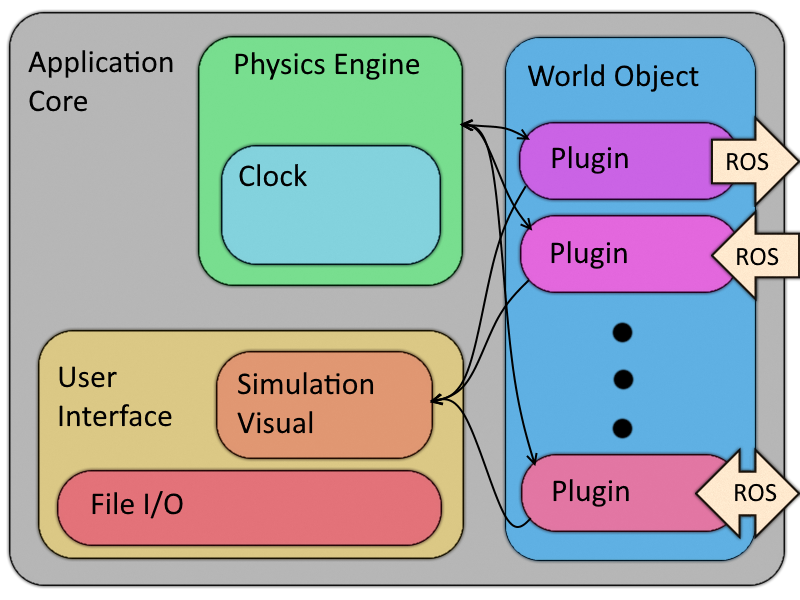
\includegraphics[width=0.75\textwidth]{./images_design/sysarch}
\end{center}
\caption{A visual representation of the system architecture, including basic data paths\label{fig:systemdiagram}}
\end{figure}

\subsection{Application Core}
The Application Core has the job of organizing the rest of the system. It connects all of the events generated by the other components and keeps track of all simulated objects. It is also responsible for adding and removing simulated objects when commanded to.

Explained in more detail below, anything simulated in the application can be represented in the World Object class. The World Object exposes functions to
\begin{itemize}
	\item Add/Remove itself from the physics engine
	\item Obtain its Models for drawing on screen
	\item Obtain its list of Properties
\end{itemize}

Models and Properties are fully defined below as well.

\subsection{Physics Engine}
The Physics Engine is the backbone of the simulation. The main purposes of the Physics Engine are
	\begin{itemize}
		\item Track what objects are part of the simulated world
		\item Step the simulated world at a regular rate
		\item Notify simulated objects when the world updates
	\end{itemize}
Forces can be applied to the simulated objects at any point in time, by any part of the application. The Physics Engine does not concern itself with where the forces originate, just the effects of them.
 
\subsection{User Interface}
The User Interface consists of all portions of the UI which are not the visualization of what is actually being simulated. The UI is responsible for things like providing the user with ways to load and save files, start and stop the simulation, and edit the properties of the simulated objects.

While the visualization of the simulated activity is, technically speaking, part of the UI, it is connected to the rest of the UI through a single interface. This allows it to be developed independently and means the rest of the UI should be agnostic to the details of how it looks and behaves. We will reference the visualization in this document with terms such as "World Visual", or "Visualization Widget".

\subsection{World Visualization}
The World Visualization is a widget in the UI which is responsible for portraying the simulated activity. Its communication is strictly with the general UI, as it is a child object of it. The UI is expected to tell this visual when objects are added and removed, as well as what models belong with those objects.

\subsection{File Read/Write}
The File Read/Write component is utilized by the general UI. When the user selects a file, the Read/Write component loads or saves a world object or collection of world objects in that file. If the file is malformed, it returns an error that the UI can display. File handlers are loaded from plugins on startup; the base project includes a save/load handler which utilizes JSON format, and a loader which can convert images to sets of World Objects.

\subsection{Plugin System}
The Plugin System keeps the core application logic separate from the specific capabilities of the simulated objects. Plugins provide the components which make up the objects simulated. Using this design allows users to write their own components for the simulation if some desired feature is missing.

\section{Technologies Overview}
\subsection{C++}
	The entire application is written using the C++ programming language. Reference material for the syntax and libraries provided as part of the language can be found at \url{http://en.cppreference.com/w/}. The most recent standard used by this project is C++11.
	
\subsection{Qt}
	Qt is a cross-platform development framework and library. It is utilized in this project for a couple of specific features it provides
	\begin{itemize}
		\item Event Loop
		\item QObjects
		\item Signals and Slots
		\item Plugins
		\item Widgets Library
		\item Graphics Framework
	\end{itemize}
	Information about the project can be found at \url{http://doc.qt.io/}. Some of the core concepts of these features are described in the following sections.
	
	An example containing QObjects and Signals and Slots can be seen in listing \ref{lst:qobjexample} below.
	
\subsubsection*{Event Loop}
	The central part of Qt is the Event Loop. When a Qt application is started, it generally enters an event loop which spins during idle time. When an event happens, it is queued until the start of the next iteration of the event loop. During each iteration of the event loop, all pending events are delivered to their receivers to be handled.
	
	\begin{lstlisting}[caption={Pseudocode for the Qt Event Loop}]
while(application_running)
{
	for(event in event_queue)
		handleEvent(event)
	Remove handled events
}
	\end{lstlisting}
	
	Many events are user-generated by actions such as clicking buttons, typing text, and resizing windows. Other events may take the form of cross-thread communication through Signals and Slots.
	
\subsubsection*{QObject}
	QObjects are the base type of anything residing in the Qt event framework. Similarly to how all Java types inherit Object, all Qt objects inherit QObject. There are two parts to QObject inheritance.
	\begin{enumerate}
		\item Inheriting QObject will add a number of common functions, signals, and slots to a type. When QObjects are instantiated, they can be given a parent QObject. When a parent QObject is destroyed, it will automatically destroy all of its children.
		\item The Q\_OBJECT macro must be placed in the \lstinline|private| portion of the class definition. At compile time, the Qt Meta Object Compiler (or MOC) is run before the standard C++ compiler. The MOC finds this macro and other Qt-specific keywords and generates standard C++ files which a normal compiler, such as g++, can use.
	\end{enumerate}
	
	Limitations on inheritance of QObject
\begin{enumerate}
	\item QObject cannot be inherited in a templated class
	\item If multiple types are inherited, QObject (or a type that isa QObject) must be the last type inherited
	\item QObject cannot be virtually inherited, so the diamond inheritance problem cannot be resolved if all types are QObjects
\end{enumerate}
	
\subsubsection*{Signals and Slots}
Signals and Slots allow programmers to define custom events and event handlers in their objects. 

A Signal is a public method of a QObject which has no definition. (The definition is added by the MOC). Instantiated QObjects can emit signals at any point in time. Signals may have parameters, and when the object emits a signal with parameters, it will fill them with data.

A Slot is a public, protected, or private method of a QObject. It must have a full definition just like any other method. (In many cases, it can be treated exactly as if it were a regular method.)

There are two main limitations on Signals and Slots
\begin{enumerate}
	\item All parameters MUST be pass-by-value. This allows all data to be copied, preventing race conditions when signals trigger slots in other threads.
	\item Custom types passed as parameters in signals and slots must be known to the Qt Meta-Object System. See documentation on the qRegisterMetaType() function for more information on how this works.
\end{enumerate}

At runtime, applications can connect the signals of instantiated QObjects to the slots of any other instantiated QObjects. When a QObject emits a signal, any slots that it is connected to will be called.


\begin{lstlisting}[language=C++, caption={Example of QObjects with parenting, Signals and Slots, and connections.\label{lst:qobjexample}}]
class foo : public QObject
{
	Q_OBJECT
public:
	//Construct with optional parent QObject
	foo(QObject* parent=nullptr) : QObject(parent){}

//Keyword known to MOC
//All signals are public methods
signals:
	void somethingHappened();
	void otherThingHappened(int);

//Another MOC keyword. Slots can be public, private, or protected
public slots:
	void reactToAnotherThing(int x)
	{
		cout << "Another thing: " << x << endl;
	}
};

class bar : public QObject
{
	Q_OBJECT
public:
	//Construct with optional parent QObject
	bar(foo* parent) : QObject(parent)
	{
		//Connect events between objects
		//Note that events and handlers have the same function signature	
		
		//When somethingHappened() is emitted by 'parent'
		//Do reactToSomething() in 'this'
		connect(parent, &foo::somethingHappened,
		        this, &bar::reactToSomething);
		
		//When otherThingHappened() is emitted by 'parent'
		//Do reactToOtherThing() in 'this'
		connect(parent, &foo::otherThingHappened,
		        this, &bar::reactToOtherThing);
		
		//When anotherThingHappened() is emitted by 'this'
		//Do reactToAnotherThing() in 'parent'
		connect(this, &bar::anotherThingHappened,
                parent, &foo::reactToAnotherThing);
	}

//Keyword known to MOC
//All signals are public methods
signals:
	void anotherThingHappened(int);	

//Another MOC keyword. Slots can be public, private, or protected
private slots:
	void reactToSomething()
	{
		cout << "Something happened!" << endl;
	}
	
	void reactToOtherThing(int x)
	{
		cout << "Reacting to other thing: " << x << endl;
		
		//Send a signal back to 'parent' object
		emit anotherThingHappened(x+1);
	}
};

int main()
{
	//Put a 'bar' on the
	foo* f = new foo();
	bar* b = new bar(f);
	
	//This will delete b as well because 
	//b is a child of f
	delete f;
}
\end{lstlisting}

\subsection{Box2D Physics}
The Box2D library is used as the basis of the Physics Engine for this simulation. It is a C++ library which can be used for realistic physics simulation and collision detection. The Box2D project is hosted on github at this location \url{https://github.com/erincatto/Box2D}.

When working with a Box2D simulation, there are a number of types that are used.
\begin{itemize}
	\item b2World: Container for everything being simulated and all extra simulation information. Bodies and Joints are added directly to the World to be simulated.
	\item b2Body: Container for physics information for one specific element of the simulation. Bodies are made up of any number of Fixtures, which are held relative to each other as the body moves. Bodies contain information such as mass, inertia, velocity, etc. Bodies can also be acted upon by forces or impulses.
	\item b2Fixture: Fixtures are used to attach shapes to a Body. Each fixture is used to attach a single shape.
	\item b2Shape: Abstract base type of any shape. Various shapes are supported by Box2D, but this project utilizes mainly b2PolygonShape and b2CircleShape.
	\item b2Joint: Joints are used to constrain how bodies move relative to each other. Many types of joints exist in Box2D, some examples are rigid, revolute, prismatic, and motor.
\end{itemize}

\subsection{ROS}
As mentioned a number of times previously, this simulation supports communication with external applications through ROS, the Robotics Operating System. Information on ROS can be found at \url{http://www.ros.org/}. The version of ROS targeted for this project is ROS 2 Ardent Abalone.

The core application itself has minimum communication through ROS, it mainly starts a ROS listener thread so that messages can be received. The bulk of the message sending and receiving is done by the plugin components which make up the objects being simulated. There are two messages sent from the core application -- A timestamp message to indicate the time passed in the simulation and joystick control messages from the virtual joystick.

\newpage
 \section{Architecture and System Design} 	
 \subsection{Design Decisions}
  	The simulation underwent a number of design changes during its development. This section will discuss what drove the major design decisions associated with this project.
 \subsubsection*{User Experience}
	Because this application is mainly for students just being introduced to robotics and will be a tool for education, we wanted to make the simulator as user friendly as possible. We decided to try for a video game-like feel, as most individuals are familiar with video games which would make it easy to learn. 
	
	The biggest design decision we had to make for the user experience aspect of the project was whether we wanted to use a single window for everything (simulation, robot builder and map builder) or if we wanted to have multiple windows. We began with a few concepts and wire frames. 

\begin{figure}
\begin{subfigure}{0.5\textwidth}
	\begin{center}
	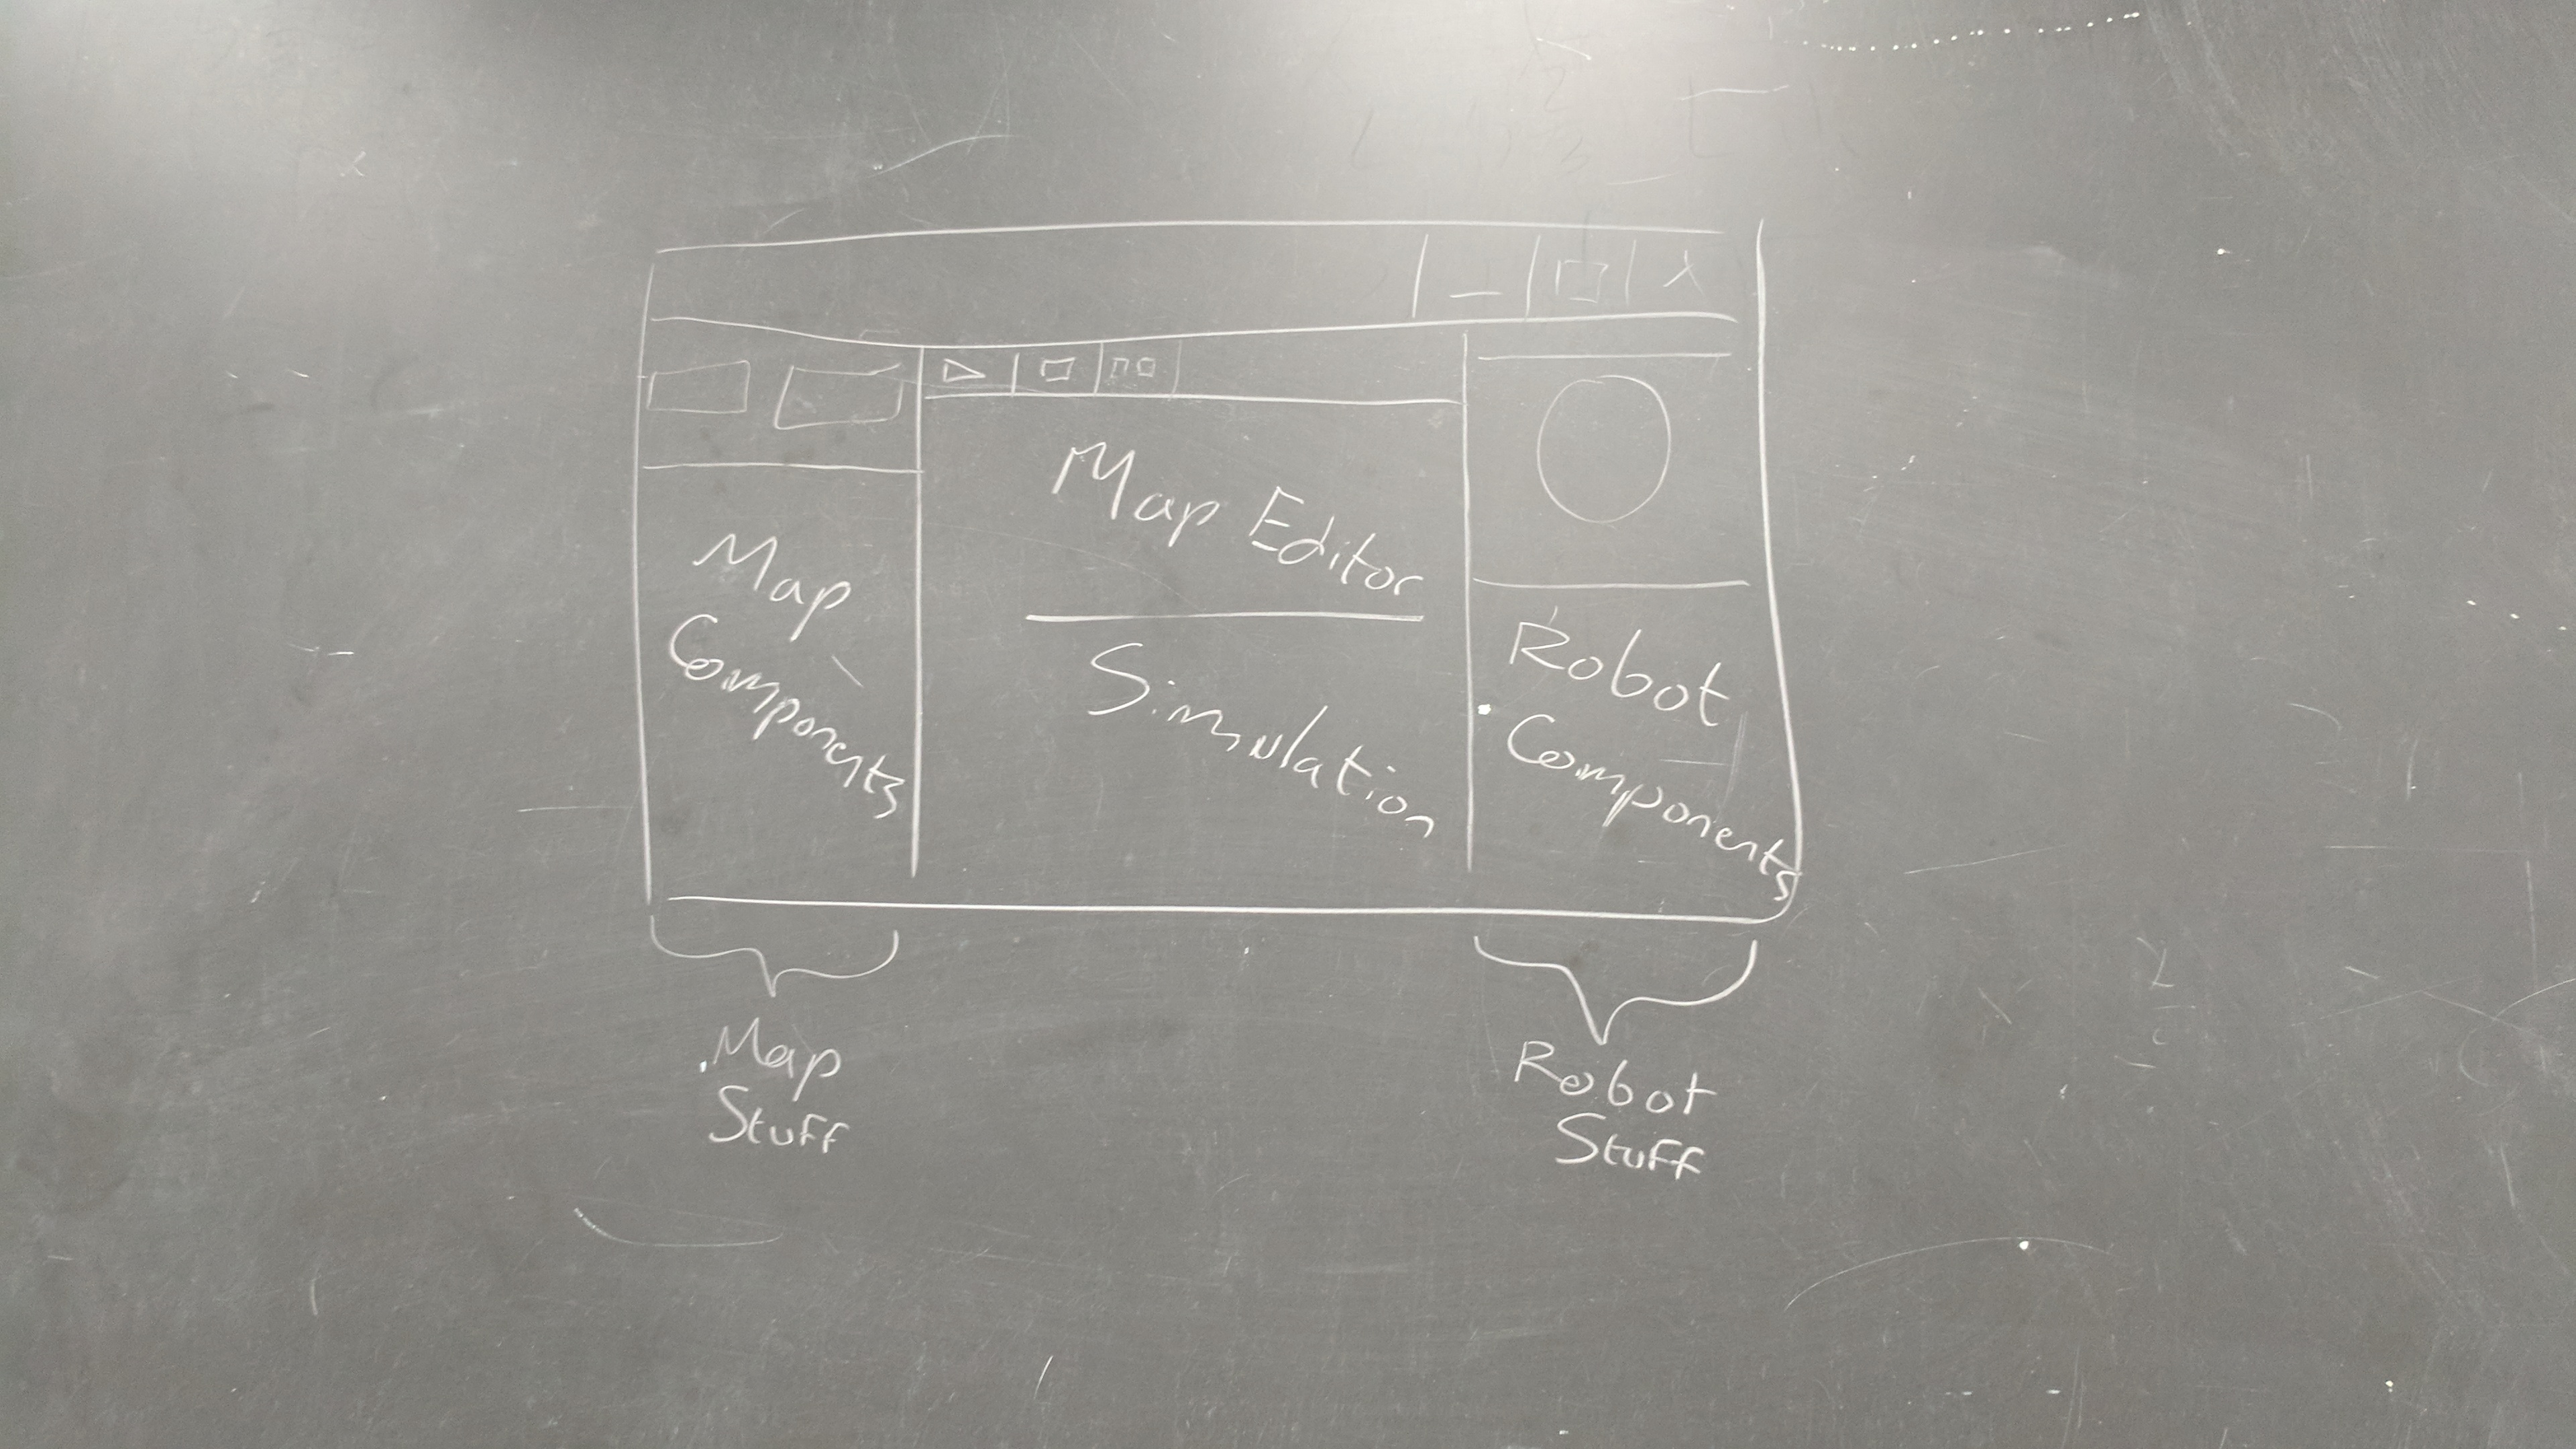
\includegraphics[width=0.9\textwidth]{./images_design/Sams.jpg}
	\caption{Single Window Concept}
	\label{fig:singlewindowconcept}
	\end{center}
\end{subfigure}
\begin{subfigure}{0.5\textwidth}
	\begin{center}
	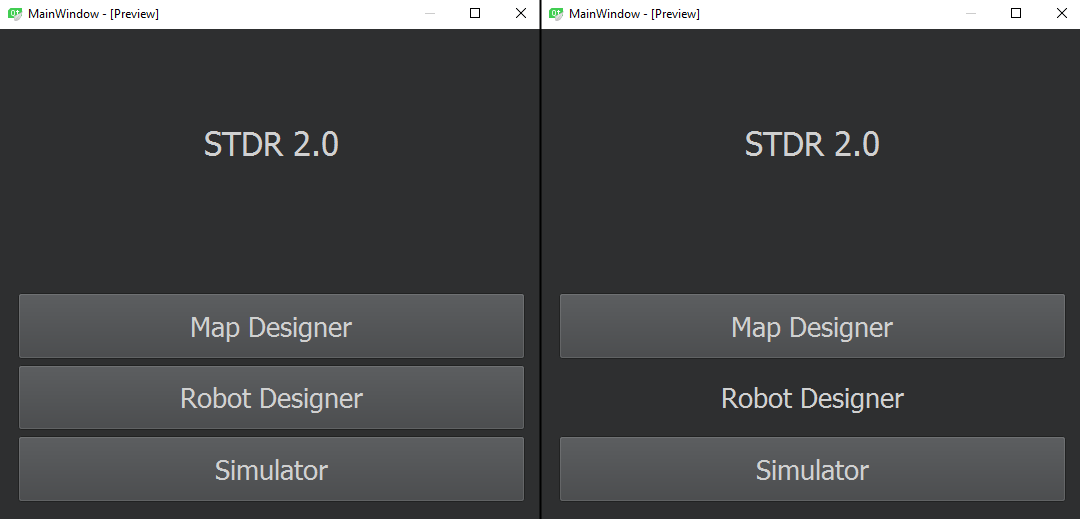
\includegraphics[width=0.9\textwidth]{./images_design/MainScreen.png}
	\caption{Multi-Window Start Window}
	\label{fig:mwindowStart}
	\end{center}
\end{subfigure}

\begin{subfigure}{0.5\textwidth}
	\begin{center}
	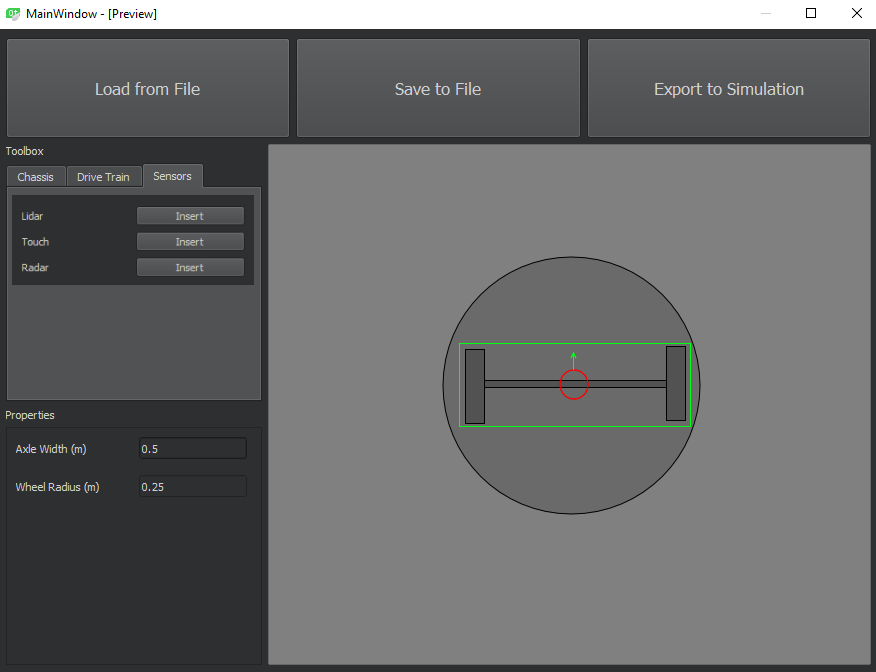
\includegraphics[width=0.9\textwidth]{./images_design/RobotDesign.png}
	\caption{Multi-Window Robot Designer}
	\label{fig:mwindowRobot}
	\end{center}
\end{subfigure}
\begin{subfigure}{0.5\textwidth}
	\begin{center}
	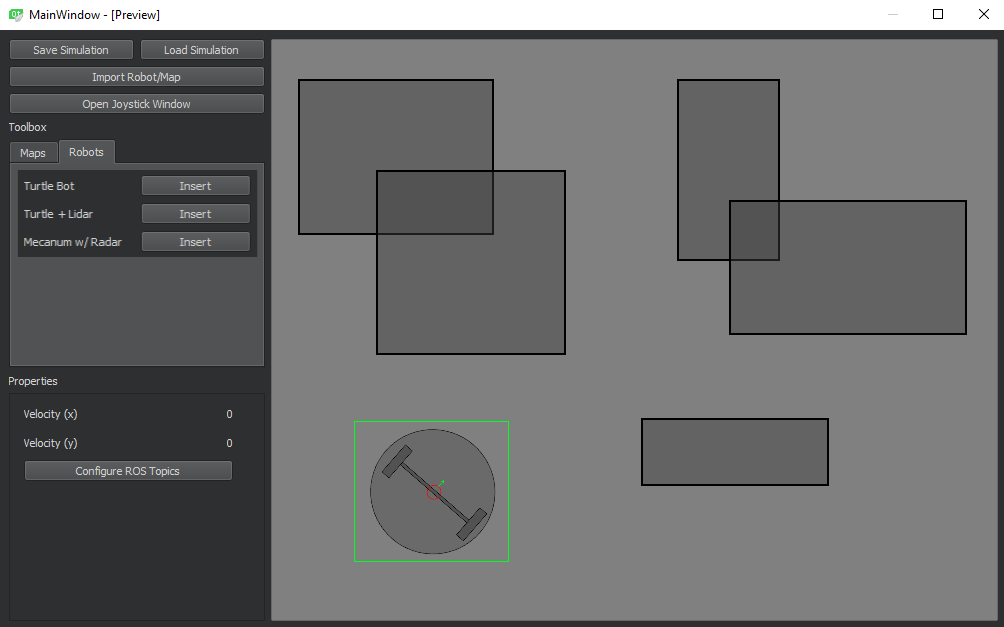
\includegraphics[width=0.9\textwidth]{./images_design/Simulation.png}
	\caption{Multi-Window Simulation}
	\label{fig:mwindowSimulation}
	\end{center}
\end{subfigure}
\caption{Example UIs presented to the Client}
\end{figure}
	
	The chalkboard drawing \ref{fig:singlewindowconcept} shows an early concept for a single window interface, while the wireframes \ref{fig:mwindowStart}, \ref{fig:mwindowRobot}, and \ref{fig:mwindowSimulation} show an idea for a multiple window interface. 

We chose to go with the single-window application both because it looks 'cleaner' and because there would be little advantage to building our application with multiple windows. It is anticipated that the user would not need to use the designer during a simulation, or the simulation during the design process; so it makes little sense to make them accessible simultaneously.  
 
 
 \subsubsection*{User Interface}
 	When building a cross-platform user interface in C++, there are only a few options available. When discussing this, the following ideas were brought up: Pure OpenGL, Qt QML, and Qt Widgets. The final decision was Qt Widgets, which will be discussed below.
 	
 	A pure OpenGL solution was not selected due mainly to the difficulty of implementation and the amount of work that would have to go into a UI of that nature. If using Qt were not an option, pure OpenGL may have been selected; however, having the Qt library available makes it hard to justify the amount of extra development that a pure OpenGL solution would add.
 	
 	When writing a UI in Qt, there are two main options for the core library: Widgets and QML. Qt Widgets has been around longer and is generally used to produce applications that look and feel 'like a desktop program'. The Widgets library contains many commonly used pieces which can be organized into a UI, similarly to how C\# Forms or Java Swing works. Qt QML is a newer library which is being actively developed with Qt. QML separates the UI entirely from the business logic by running the UI in a custom javascript interpreter. The main advantages to QML are that it's very easy to develop QML UIs without any business logic and it's currently receiving the bulk of support in new versions of Qt. QML would have been the first choice for the project UI, but it is difficult to use on a freshly installed system. Widgets projects require just a set of shared objects to run, but QML projects require a number of shared objects as well as some basic QML code files which are parsed at runtime. These additional files are not usually present in the base library installation of Qt, so using QML would have meant that the end user would need to resolve extra dependencies to run the application.
 	
 	\subsubsection*{World Visualization}
 	Within the Qt Widgets library, there are a number of different ways build a widget with a drawing canvas that shapes can be shown on. The most primitive method is to create an OpenGL drawing window which is contained in the widget. The other main option is to use the Qt Graphics Framework, which is an abstraction layer for drawing 2D objects on a background with OpenGL.
 	
 	Again, it was decided that the pure OpenGL solution would add unnecessary development time, and an alternative should be used. Not only does the graphics framework provide easy methods for drawing primitive shapes on a canvas, but it also allows for parent-child relationships between the models, which in turn allows shapes to be defined with relative transforms to each other instead of everything needing to be in world coordinates.
 	
 	\subsubsection*{Physics}
 	One of the main failings of STDR was its lack of a physics engine. It was decided early on that a known physics engine should be used, or one should be written for this project so that at least basic collision detection could be simulated.
 	
 	A number of different engines were investigated, including Box2D and Chipmunk2D. In the end, Box2D was chosen because it is simple and lightweight while also providing all of the functionality necessary for this simulator. Other physics engines would have been too bulky or difficult to use, and writing a custom physics engine would have extended the development considerably and likely would have resulted in worse performance.

	\subsubsection*{Non-Kinematic Solution}
	The original STDR operated using standard mobile robot kinematic formulas. Kinematics, and Inverse Kinematics, are systems of equations which can be used to map robot actions from control space to physical space and from physical space to control space. For example, in a kinematic solution, the robot control code may publish wheel velocities. The simulator, upon receiving these velocities, the simulator uses the forward kinematic equations of the robot to determine the overall velocity of the craft. This velocity can be used in a physics simulation.
	
	Kinematics equations of mobile robots are very specific to the driving base in use. Some commonly known ones are the Differential Drive, Mecanum Drive, and Ackermann Steer.
	The original plan for this project was to take a similar approach, using the forward kinematic formulas to produce overall craft velocities that Box2D could use. At one point, the Client mentioned that it would be cool if we didn't have to explicitly define kinematic equations for each drive system, but could let the user place wheels on a robot frame and drive it. At the time, none of the team were aware of how this could be properly simulated. The biggest issue with simulating this kind of a system is that it would be difficult to determine the proper forces to apply to keep 'no slide' conditions on a wheel. 'No slide' constraints are limitations which prevent the wheel from moving perpendicular to its intended direction of travel.
	During the implementation of the Touch Sensor Ring plugin, one team member stumbled across a tutorial outlining how to use Box2D to simulate a top-down steered vehicle that a user could drive. The tutorial showed how using different physics bodies for each wheel would allow the simulation to negate any forces which would cause the wheel to slide perpendicular to its intended direction of motion. 
	At this point, the decision was made to completely rework how robots are defined within the application. Rather than load plugins which have the kinematic equations for specific wheel bases, the user will load plugins which define how specific wheels move. Those wheels will be placed on robot frames and can apply whatever forces are necessary to constrain robot movement as they should.
	
	\subsubsection*{Single vs. Multiple Threads}
	One of the early design choices was the do as much processing in parallel as possible. It is reasonable that this project will be used to simulate large worlds with many robots, and each robot could have many sensors on it. The idea was that if all sensor calculations could be computed in parallel, the simulation would be less likely to lag behind real-time under these circumstances.
	During implementation of the Touch Sensor Ring plugin two things became evident:
	\begin{itemize}
		\item It would be more trouble than it's worth to use Box2D safely in a multithreaded application
		\item Sensor calculations will likely be fast enough that they won't impact the simulation significantly
	\end{itemize}
	After these realizations occurred, the decision was made to keep all processing in a single thread to simplify the application. The major risk to this design is that the system will lag behind real-time; however this should not affect simulations, just the observation of them. It is planned that the simulator will publish timestamp messages so that control code which relies on the passage of time can correctly account for any lag in the system.
%\section{Notable Algorithms} 
 %\subsubsection{Importing Images}

 \newpage
\subsection{Classes}
  \subsubsection*{Model}
  The Model class is a container for shapes; it is designed to be used to communicate what should be drawn on the screen. When models change or move, signals are emitted so that the image drawn can update to reflect the changes.
  
 	The UML of the Model class can be seen in UML Figure \ref{uml:model}. The Model class provides constructors to initialize it with any number of child Models and/or shapes and exposes accessor methods for both.

 \begin{figure}[h]
 	\begin{center}
 	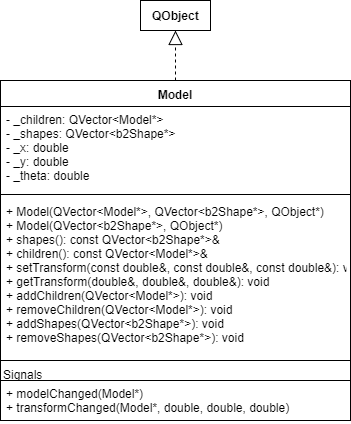
\includegraphics[scale=0.5]{./images_design/uml/Model}
 	\caption{UML of Model\label{uml:model}}
 	\end{center}
 \end{figure}  
 
 All children of a Model should exist on the heap. Upon its deletion, the Model will delete all of its children. The shapes of a Model may exist anywhere in memory, as the Model will NOT delete its shapes at any time. 
 
After construction, shapes and children models can be added and removed with the four functions
 \begin{itemize}
 	\item addChildren()
 	\item removeChildren()
 	\item addShapes()
 	\item removeShapes()
 \end{itemize} 
 
 Calling any of these functions will result in the modelChanged() signal being emitted. This design allows the UI to do the minimum amount of re-rendering necessary when part of a model updates. If the renderer needs to know when to update based on children of the model, it should use the children() method to get the list of children and listen for the modelChanged() signal from each of them.
 
 The transform of the model can be accessed through getTransform() and setTransform(). Setting the transform will result in the transformChanged() signal being emitted.
 
 Figure \ref{uml:dataflow_model} depicts the series of notifications which result from moving or modifying a Model and its child Models.
 \begin{figure}[h]
 	\begin{center}
 	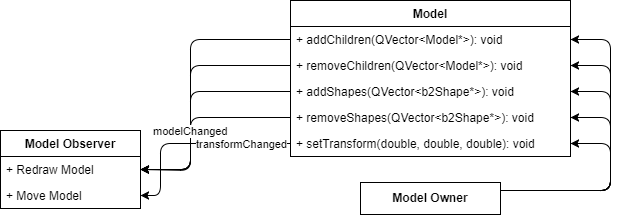
\includegraphics[width=0.75\textwidth]{./images_design/uml/DataFlow_Model}
 	\caption{Flow of data using Models. When the Model owner updates a model, any observers are notified. \label{uml:dataflow_model}}
 	\end{center}
 \end{figure}   
 
 \subsubsection*{Property}
 	Properties are variables within an object that may be modified by external sources. They are accessed through PropertyView objects, which enforce read/write rules so that internal state that should not be changed is not changed by accident. The UML Diagrams for Properties, PropertyViews, and all associated types are found in Figure \ref{uml:property}
 	
 \begin{figure}[h!]
 	\begin{center}
 	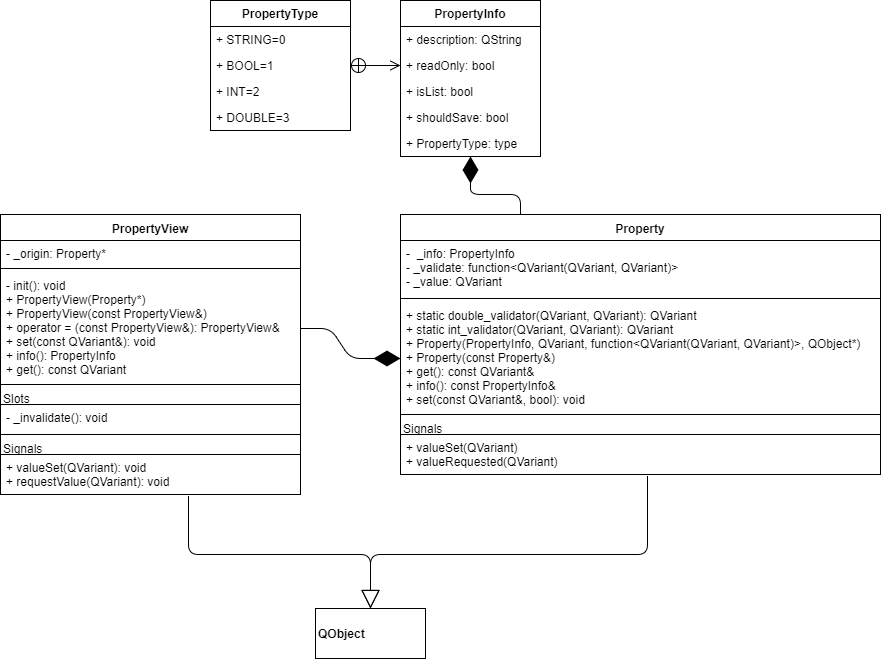
\includegraphics[width=\textwidth]{./images_design/uml/Property}
 	\caption{UML of Property and associated classes\label{uml:property}}
 	\end{center}
 \end{figure} 
 
 	A Property has three main parts
 	\begin{itemize}
 		\item Its PropertyInfo
 		\item A validation function
 		\item Its value
 	\end{itemize}
 	
 	The PropertyInfo is a container for any meta information about the Property. This contains data such as the type of the data, whether or not it's read-only, whether or not it's a list, and a description of what the Property is used for. This is intended to be used to aid a UI which displays Properties to the user. It is assigned to a Property once, at construction, and can be accessed through the info() method.
 	
 	The validation function follows the prototype \lstinline|function<QVariant(QVariant, QVariant)>| and is used to make sure that the data assigned to the Property is valid. The first parameter represents the previous value, and the second parameter is a potential new value. The function should return the new value if it is acceptable and the old value if the new one is not acceptable (Optionally, the function may change the new value to make it valid and then return it). The default validation function accepts all values. A number of basic validation functions exist as static methods of the Property class for convenience. Some of them are
 	\begin{itemize}
 		\item double\_validator()
 		\item int\_validator()
 	\end{itemize}
 	
 	The value of a property is accessed and mutated though the methods set() and get(). get() returns the current value. set() validates a new value using the validation function and stores whatever value is returned. Whenever the set() function is called, the valueSet() signal is emitted with the value that was set. This happens even if the stored value does not change. The valueRequested() signal is emitted under similar conditions, but only when the value changed because of a request from a PropertyView. This can be used by the owner to only react to external changes, allowing internal changes to not trigger any slots listening for the value change.
 	
 	The PropertyView object contains all of the same public functions as a Property; however it is constructed with only a Property, which it observes. When the set() function is called on a PropertyView, the requestValue() signal is emitted, and the original Property handles that signal and validates the new value. The valueSet() signal in a PropertyView is tied to the same signal in its observed property so that any owner of a PropertyView will know when the value changes.
 	
 	The internal slot \_invalidate() is called when the observed Property is destroyed to prevent a null reference. If any accessors are called after this happens, they will return default-constructed values. It is intended that the owner of a PropertyView will receive some indication that the PropertyView should no longer be tracked from another source.
 	
 	Figure \ref{uml:dataflow_property} shows the flow of data between properties, property owners, property views, and property observers.
 	
 \begin{figure}[h]
 	\begin{center}
 	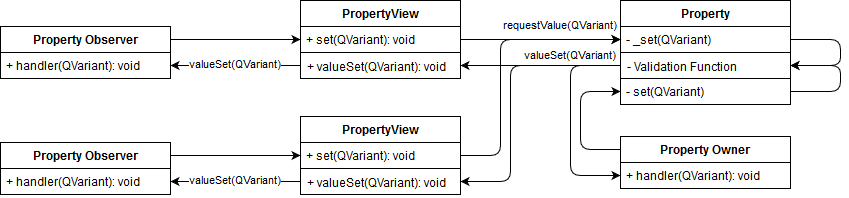
\includegraphics[scale=0.5]{./images_design/uml/DataFlow_Property}
 	\caption{Data flow of Properties, their owners, and their observers. Note that any time a value is set (Either through a PropertyView or directly) the data is validated before the new value is sent to the owner and any observers.\label{uml:dataflow_property}}
 	\end{center}
 \end{figure} 
 	
  \subsubsection*{World Object Component} \label{sec:worldobjclass}
	The main data type in this simulation is the World Object Component. For the UML diagram of a World Object Component, see Figure \ref{uml:worldobj}.
	
 \begin{figure}[h]
 	\begin{center}
 	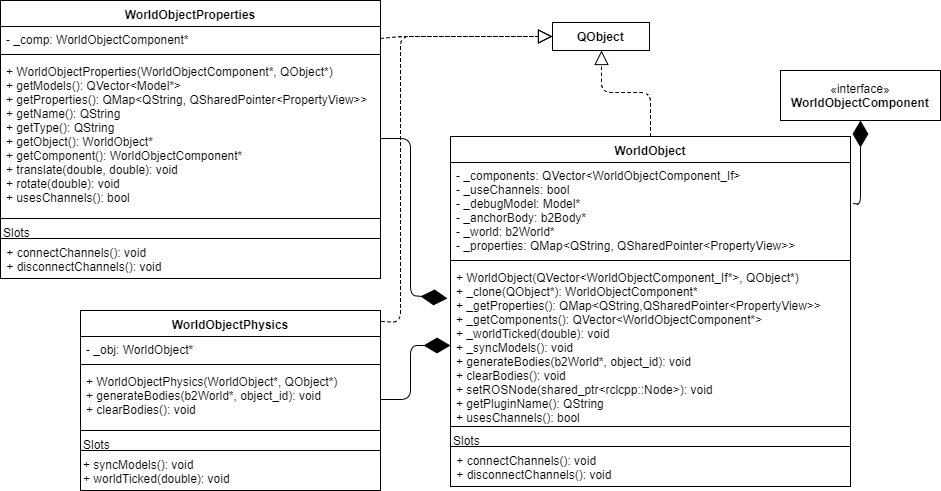
\includegraphics[scale=0.5]{./images_design/uml/WorldObj}
 	\caption{UML of World Objects, World Object Components, and associated classes\label{uml:worldobj}}
 	\end{center}
 \end{figure}
	
	It is possible that a World Object Component will use external communications, such as ROS. The usesChannels() accessor is used to determine if this is the case, and the connectChannels() and disconnectChannels() slots are used to start or stop communications.
	
	When a World Object Component is added to the physics engine, it is given access to the Box2D world. At this point, the World Object Component creates any Box2D bodies needed and set up the shapes, masses, and joints required to simulate the component. During the simulation, components can apply forces to their bodies to create movement in the world. When the World Object Component is removed from the physics engine it should destroy any joints and bodies that it has created in the current box2d world.

	The World Object Component type contains a number of methods to help integrate with the rest of the application. The main concerns are keeping track of the Models and Bodies associated with the Component and moving them around as a group when the Component is translated
	or rotated. To aid this, the methods \lstinline|registerBody()|, \lstinline|unregisterBody()|, \lstinline|registerModel()|, and \lstinline|unregisterModel()| exist as part of World Object Component. Any subclass can call these methods to add or remove handling for bodies and models. Registering either a Model or Box2D Body will move them into global space. The current transform of the Model or Body at the time of registration is assumed to be the location of that Model or Body relative to the Component (or their location in local space); upon registration, the Model or Body is moved to global space. When Bodies are registered, they can be tied to any number of Models; tying a Body to a Model means that the Model's global transform will be updated each step to match that of the Body. Bodies can also be set as the main body for the component, which means that it's location will be the location reported for the Component. If no main body is set, the Component will behave no differently, except that its location will not change due to the simulation.

	When registering and unregistering Models and Bodies, there are a couple of things to keep in mind:
	\begin{itemize}
		\item All Models should be registered during the constructor; the set of registered models should not change except during destruction
		\item Models tied to bodies are not required to be registered, and vice-versa; however, Models not tied to bodies will not move automatically, it will be up to the Component to move them during \lstinline|_syncModels()|
		\item Models and Bodies should not be destroyed until they are unregistered
		\item Models should not be destroyed while they are tied to a body
	\end{itemize}

	World Object Components also have a couple of default Properties: Name, Local X, Y, Theta, and Global X, Y, Theta. Local position is relative to any parent components; if no parent exists, then the Local position will be 0, 0, 0 at all times.

	Finally, World Object Components have a type which is assigned during construction and accessed through \lstinline|getType()|. This value is used to sort components into groups of like components.
  
	\begin{figure}
		\begin{center}
		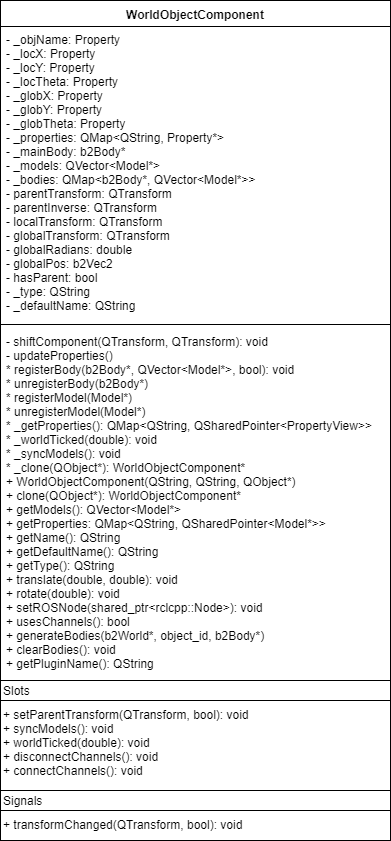
\includegraphics[scale=0.5]{./images_design/uml/WorldComponent_If}
		\caption{UML of World Component class interface\label{uml:worldcomponent_if}}
		\end{center}
	\end{figure} 

\subsubsection*{World Object}
	World Objects are a special kind of World Object Component. They are container types which hold any number of other components as children. These consolidations are the data type which is added to and removed from the simulation.

	World Objects, upon construction, consolidate all of the models and properties of their components. When getModels() or getProperties() is used to access the World Object, these consolidated lists are returned.

	Only the Simulator Core holds the reference to a World Object in the simulation. As can be seen in the UML diagram, a number of wrapper objects exist to provide specific interfaces. The WorldObjectProperties class provides an interface to a World Object which is used by the User Interface, and the WorldObjectPhysics provides the interface used by the Physics Engine. These interfaces are children (in the Qt sense) of the original World Object, so no owner of an interface needs to delete their interface when the WorldObject is removed from the simulation.
  
  \subsection{Interfaces}
  \subsubsection*{Physics Engine Interface}
  The SimulationPhysics\_If interface (UML Figure \ref{uml:phys_if}) provides the interface any Physics Engine used in this simulation must follow. It is expected that any Physics Engine will be built on Box2D.
  
 \begin{figure}[h]
 	\begin{center}
 	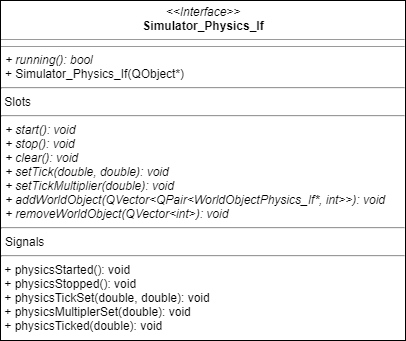
\includegraphics[scale=0.5]{./images_design/uml/Physics_Engine_If}
 	\caption{UML of Physics Engine class interface\label{uml:phys_if}}
 	\end{center}
 \end{figure}  
  
  There are four main methods for modifying the flow of the simulation and two main methods for influencing what is actually simulated.
  
  The methods for changing simulation flow are
  \begin{itemize}
  	\item start()
  	\item stop()
  	\item clear()
	\item setTick()
	\item setTickMultiplier()
  \end{itemize}
  
  The methods for adding and removing simulated objects are
  \begin{itemize}
  	\item addWorldObject()
  	\item removeWorldObject()
  \end{itemize}
  
  The Physics Engine should emit the following signals under appropriate circumstances.
  \begin{itemize}
  	\item physicsStarted()
  	\item physicsStopped()
  	\item physicsTickSet()
  \end{itemize}
  
  \subsubsection*{UI Interface}
  A UI for this simulation is expected to provide users with the following features
  \begin{itemize}
  	\item Add/Remove elements from the simulation
  	\item Start/Stop/Time Warp the simulation
  	\item Display Error messages
  \end{itemize}
  
  The UML diagram of this interface (Figure \ref{uml:ui_if}) defines the exact signals and slots that are expected for these functions.
 \begin{figure}[h]
 	\begin{center}
 	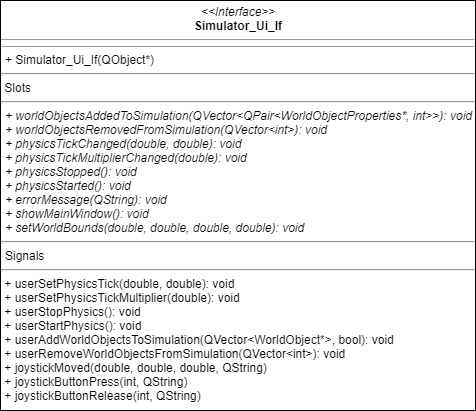
\includegraphics[scale=0.5]{./images_design/uml/Ui_If}
 	\caption{UML of UI class interface\label{uml:ui_if}}
 	\end{center}
 \end{figure}
 
 All data flow with the UI should follow a circular pattern. This means that, when the UI generates a signal, it should not update until a response has been received. This prevents the UI from getting out of sync with the rest of the application. This is the explanation for each signal having a corresponding slot. The UI should emit the signal and only update the screen when the slot is called.
 	
  \subsubsection*{View Widget Interface}
  The View Widget interface is a requirement of the specific UI written for this project. It provides a standardized way for the MainWindow UI class to update the world view widget, regardless of what drawing library that widget uses.
  
  This interface provides methods which allow
  \begin{itemize}
  	\item Setting the size of the world
  	\item Adding and removing models associated with an object
  	\item Changing how models for an object are drawn
  	\item Selecting objects and indicating selection
  \end{itemize}
  
  As with the general UI interface, the Visual Widget should not update the selected object when the user click event happens, but instead should signal that the user selected an object and wait for the objectSelected() method call.
 \begin{figure}[h]
 	\begin{center}
 	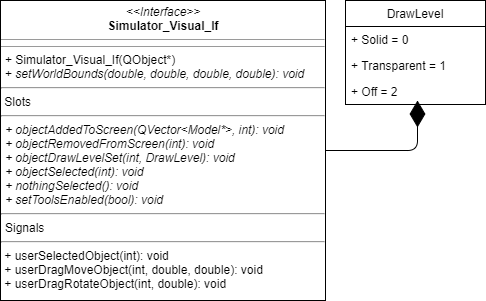
\includegraphics[scale=0.5]{./images_design/uml/Visual_If}
 	\caption{UML of Visualization widget interface\label{uml:visual_if}}
 	\end{center}
 \end{figure}
  \subsubsection*{File Handler Plugin Interface}
  File Handlers are loaded at runtime from plugin libraries following this interface. The interface should provide a set of Loaders and a set of Savers, but one or both sets can be empty. File Handler Plugins are specific to the handling of single objects or entire simulations, covered by the \lstinline|WorldObjectFileHandler_Plugin_If| and \lstinline|WorldFileHandler_Plugin_If| respectively. The loaders and savers returned by the plugin also cover the same category of files.
   \begin{figure}
 	\begin{center}
 	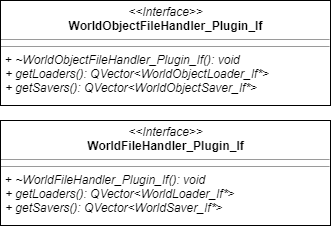
\includegraphics[scale=0.5]{./images_design/uml/FileHandler_If}
 	\caption{UML of File Handler interface\label{uml:filehandle_if}}
 	\end{center}
 \end{figure}
 File Loaders (Figure \ref{uml:fileload_if}) allow a three step process when loading files:
 \begin{enumerate}
	\item Check that a file is the proper format
	\item Prompt the user for settings
	\item Load the file, using the settings from the most recent prompt
 \end{enumerate}
 These steps are covered by the three methods of a file loader:
 \begin{enumerate}
	\item \lstinline|canLoadFile()|
	\item \lstinline|getUserOptions()|
	\item \lstinline|loadFile()|
 \end{enumerate}
 During the first step, the loader should verify that the file exists and read enough of it to determine that it is the correct format. Simply checking for the correct extension is not enough.

 If the loader needs to get information from the user to load the file, this can be done with a dialog prompt in the second step. It should not be done in the third step, because that step may not be run in the main thread.

 In the third step, the loader should open the file and load any WorldObject(s) found. The user settings chosen in the most recent prompt from \lstinline|getUserOptions()| should be used, if any are needed.

 During any of these steps, it is acceptable for the loader to throw an exception if unexpected situations are encountered.

 \begin{figure}[h]
	\begin{center}
	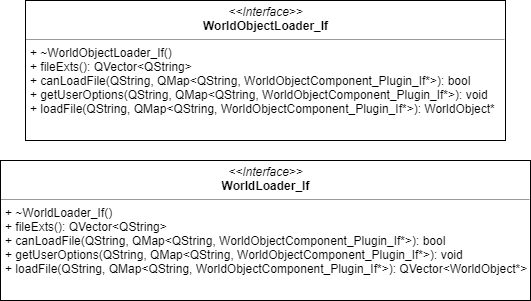
\includegraphics[scale=0.5]{./images_design/uml/Loader_If}
	\caption{UML of Plugin interface\label{uml:fileload_if}}
	\end{center}
\end{figure} 

 File Savers (Figure \ref{uml:filesave_if}) are much simpler, they have a single \lstinline|saveFile()| method which writes out the requested file.

 \begin{figure}[h]
	\begin{center}
	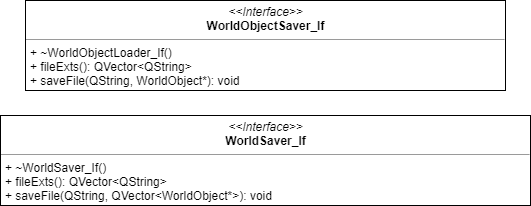
\includegraphics[scale=0.5]{./images_design/uml/Saver_If}
	\caption{UML of Plugin interface\label{uml:filesave_if}}
	\end{center}
\end{figure}

 Both File Savers and Loaders have the \lstinline|fileExts()| method which returns a vector of strings. Each of these strings should be a single group of file types that go together, following the Qt File Dialog format. For example, a file loader that can load any image file might return \lstinline|"Images (*.jpg *.png *.bmp)"|, and one that can process JSON or XML files might return \lstinline|"JSON Files (*.json)"| and \lstinline|"XML Files (*.xml)"|.

  \subsubsection*{World Object Component Plugin Interface}
  This interface defines how plugins containing World Object Components should look. Plugins are loaded using the Qt Plugin Loader; information on the plugin system can be found at \href{http://doc.qt.io/qt-5/plugins-howto.html#the-low-level-api-extending-qt-applications}{http://doc.qt.io/qt-5/plugins-howto.html}. 
  The only purpose of these plugins is to create instances of the World Object Component they contain. These instances will be cloned or added into World Objects.
 \begin{figure}[h]
 	\begin{center}
 	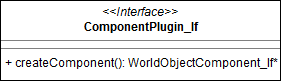
\includegraphics[scale=0.5]{./images_design/uml/ComponentPlugin}
 	\caption{UML of Plugin interface\label{uml:componentplugin}}
 	\end{center}
 \end{figure} 
 
 \subsection{Data Flow}
 All data flows between the major system components through Qt Signals and Slots. There are four main events which drive data flow
 \begin{itemize}
 	\item World Object Added
 	\item World Object Removed
 	\item Simulation Ticked
 	\item Plugin Receives External Input
 \end{itemize}
 
 \subsubsection*{World Object Added}
 	World Object additions are generally initiated by the UI. When the user wants to add an Object to the simulation, the UI signals to the core indicating what Object should be added. The core copies the World Object and stores the copy with an index. The Object and its index are sent back to the UI and Physics engine wrapped in interfaces which can be used to access methods of the new World Object.
 	
 	\begin{figure}[h]
 		\centering
 		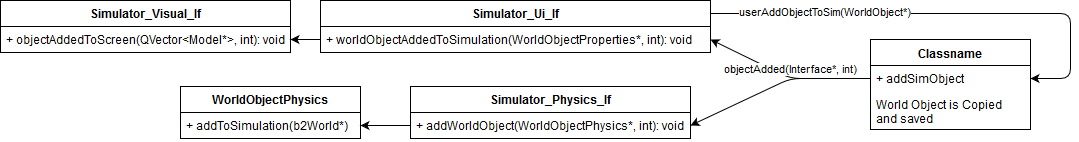
\includegraphics[width=\textwidth]{./images_design/uml/event_addObject}
 		\caption{Data flow when a new object is added to the simulation\label{uml:addevent}}
 	\end{figure}
 	
 	When the Physics engine receives a new World Object, it passes the b2World object
of the simulation to it so that the Object can add bodies and shapes to the physics engine.

	When the UI receives a new World Object, it passes the object's Model to the world view to be drawn and caches the list of object Properties. When the user selects this Object, those Properties are displayed for viewing and editing.
	
 \subsubsection*{World Object Removed}
 The process of removing a World Object is very similar to that of creating one. The UI signals to the core that the user would like to remove an Object; this Object is identified by the index that was assigned when it was added to the simulation. The core then signals back to the UI and Physics that this Object is removed and deletes the associated Object from the heap.
 
 	\begin{figure}[h]
 		\centering
 		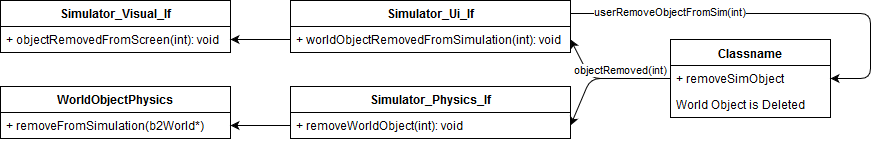
\includegraphics[width=\textwidth]{./images_design/uml/event_removeObject}
 		\caption{Data flow when an object is removed from the simulation\label{uml:removeevent}}
 	\end{figure} 
 
 When the Physics engine receives this signal, it passes the b2World to the Object again so that the Object can remove any Box2D bodies and joints that it created.
 
 When the UI receives this signal, it un-caches the Object's list of Properties and notifies the world view widget to stop drawing the Models associated with the object.
 
 \subsubsection*{World Ticked}
 World ticks are generated by the physics engine on a timer. The default tick rate is 30 per second, and each tick moves the simulation forward $\frac{1}{30}$ of a second.
 
 When a Component of an Object receives this signal, it may update its own Model, which would redraw the screen with the change. Additionally, Components can take this moment to modify the simulation by applying forces on their Box2D bodies or send messages to external applications through ROS.
 
  	\begin{figure}[h]
 		\centering
 		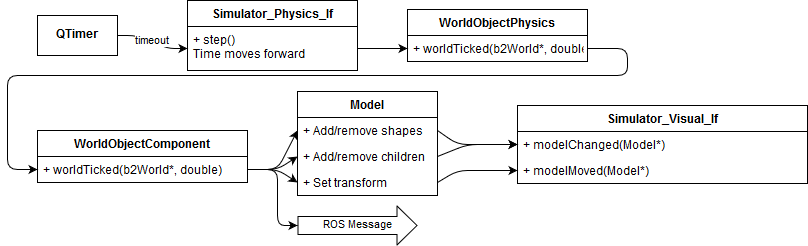
\includegraphics[width=\textwidth]{./images_design/uml/event_tick}
 		\caption{Data flow of a simulation tick\label{uml:tickevent}}
 	\end{figure}
 
 \subsubsection*{External Communication}
 The most common example of external communication is robot control code signaling that wheel velocities should change. When World Object Components receive an external communication of this nature, they can apply forces on their associated Box2D body to affect the simulation and update their models. This change will be applied on the next tick to happen after the force is applied.
 
  	\begin{figure}[h]
 		\centering
 		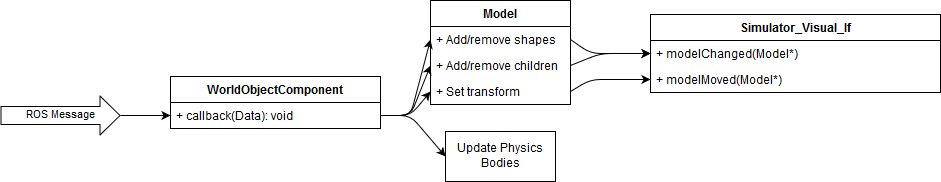
\includegraphics[width=\textwidth]{./images_design/uml/event_data}
 		\caption{Data flow of a ROS message being received\label{uml:dataevent}}
 	\end{figure}
 
\subsection{Simulator Core}

\subsubsection*{Technologies Used}
\begin{itemize}
	\item Qt
\end{itemize}

\subsubsection*{Overview}
The simulator core is, as the name suggests, the main piece of the simulation. It organizes the other parts of the system and ensures that data flows in the correct paths. The main purpose of the simulator core is to connect the UI to the Physics engine and keep them synchronized so that what's shown on screen reflects what's simulated in the physics engine. See UML Figure \ref{uml:simcore} for a list of data members and functions in the simulator core. The specific data connections set up by the core are shown in Figure \ref{uml:dataflow_simcore}.

 
 \begin{figure}[h]
 	\begin{center}
 	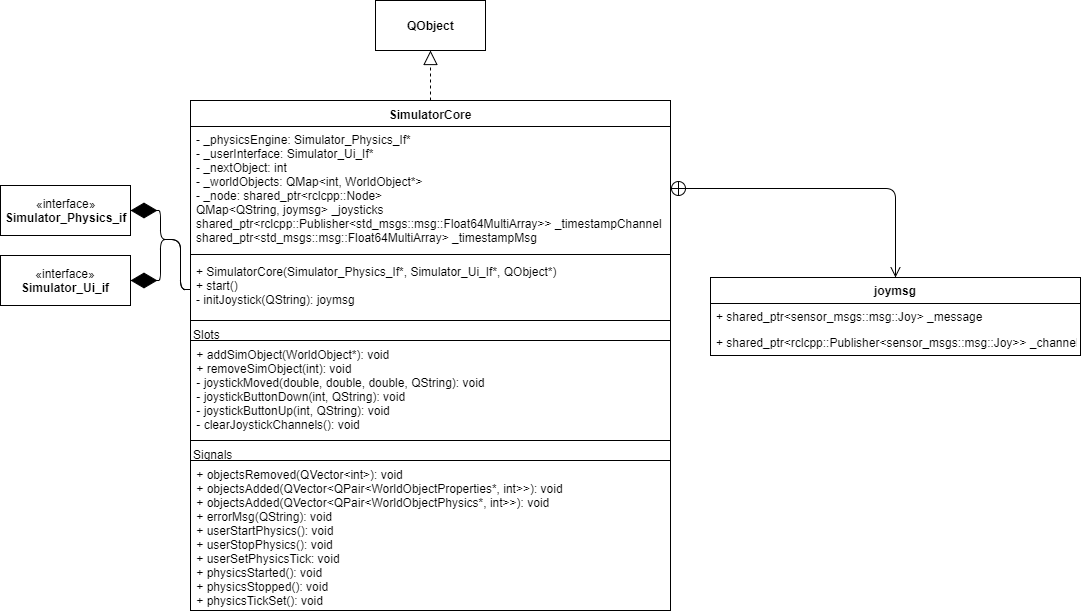
\includegraphics[scale=0.5]{./images_design/uml/SimCore}
 	\caption{UML of Simulator Core\label{uml:simcore}}
 	\end{center}
 \end{figure}

 \begin{figure}[h]
 	\begin{center}
 	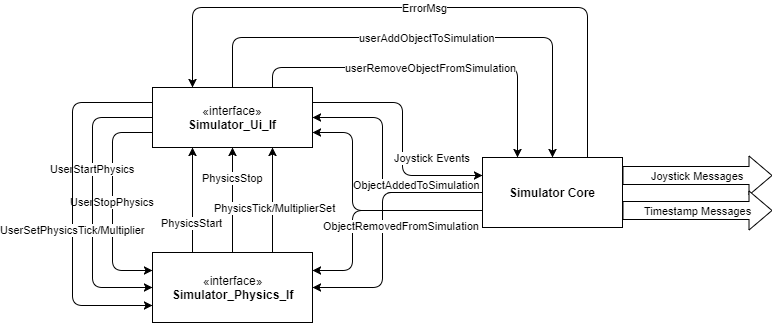
\includegraphics[scale=0.5]{./images_design/uml/DataFlow_simcore}
 	\caption{Data connections created by the Simulator Core\label{uml:dataflow_simcore}}
 	\end{center}
 \end{figure} 

\subsubsection*{Design Details}
\begin{itemize}
	\item World Objects are assigned an unsigned index when they are added. These indexes count up from 1. 0 can safely be used elsewhere as a placeholder for None.
	\item Added World Objects are cloned, so the original copy must be deleted correctly wherever it exists.
	\item The Simulator\_Ui\_If* and Simulator\_Physics\_If* that are used to construct the core will be deleted by the core's destructor.
\end{itemize}

\subsection{Physics Engine}

\subsubsection*{Technologies  Used}
\begin{itemize}
	\item Qt
	\item Box2D
\end{itemize}

\subsubsection*{Component  Overview}
The physics engine is responsible for updating the world state at regular intervals. When objects are first added to the world, they should be initialized in the physics engine, and until they are removed from the world they should be simulated along with the rest of the objects. The physics engine should be capable of starting, stopping, changing rate, and adding or removing an object while in any state. The current physics engine is the 'BasicPhysics' object found in UML Figure \ref{uml:physics}. The interface that it follows is found in UML Figure \ref{uml:phys_if}

 \begin{figure}[h]
 	\begin{center}
 	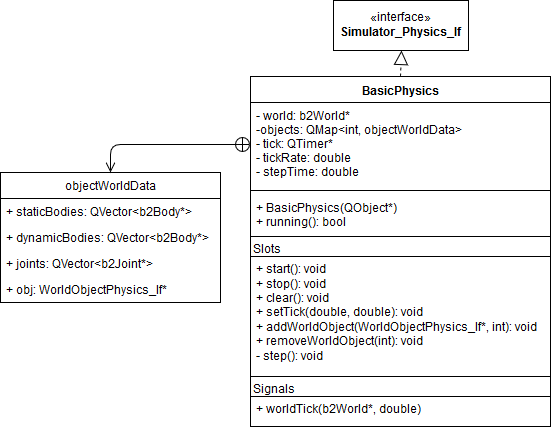
\includegraphics[scale=0.5]{./images_design/uml/BasicPhysics}
 	\caption{UML of Physics Engine\label{uml:physics}}
 	\end{center}
 \end{figure}

 \begin{figure}
 	\begin{center}
 	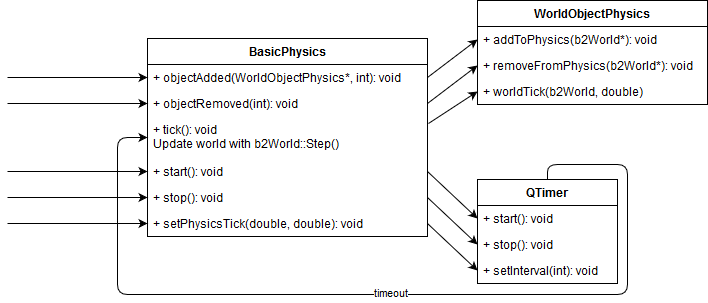
\includegraphics[scale=0.5]{./images_design/uml/DataFlow_physics}
 	\caption{Data Flow in Physics Engine\label{uml:dataflow_physics}}
 	\end{center}
 \end{figure}

\subsubsection*{Design Details}
\begin{itemize}
	\item Two things happen on every tick: The world updates (b2World::Step), then all world objects are notified of the tick
	\item The QTimer is started and stopped with QTimer::start, QTimer::stop. This means that if processing a tick takes longer than the set interval, the timer events will start to stack up. It may be necessary to look at a different method of ticking to prevent this.
\end{itemize}

\subsection{User Interface}
\subsubsection*{Technologies Used}
\begin{itemize}
	\item Qt
	\item Qt Widgets
\end{itemize}
\subsubsection*{Overview}
The user interface implemented for this project has the following features
\begin{itemize}
	\item Start/Stop simulation
	\item Time Warp simulation
	\item Add/Remove simulated item
	\item Load/Save simulation states
	\item Save a screenshot of the simulation
\end{itemize}

\hrule
TODO
\begin{itemize}
	\item Design mode - design, build, document, and test
	\item Time Warp
	\item Resetting
	\item Saving/Loading full simulations
	\item Loading Image files
\end{itemize}
\hrule

 \begin{figure}
 	\begin{center}
 	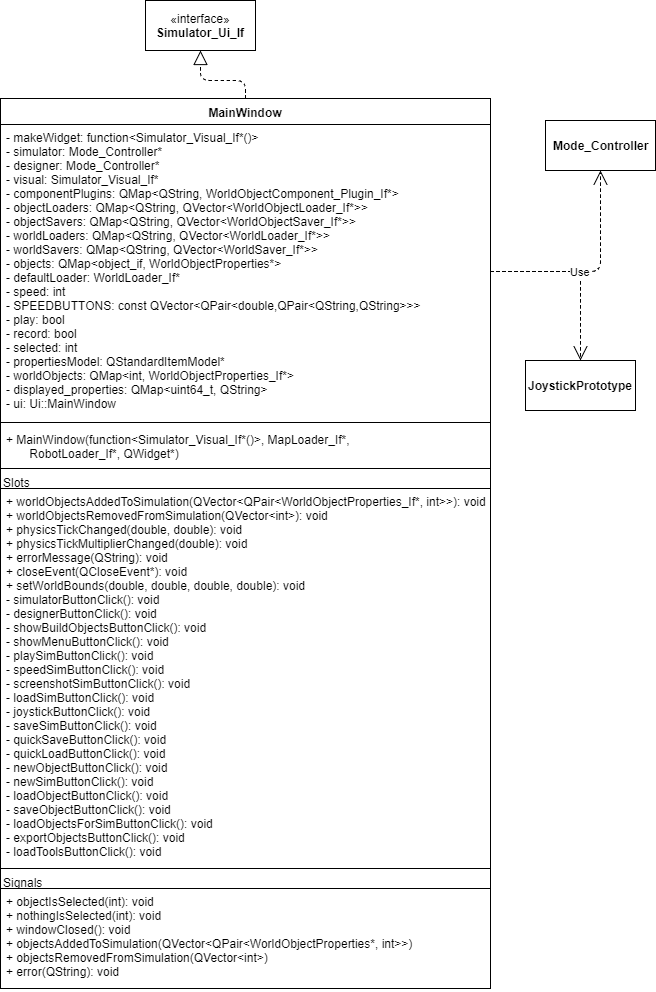
\includegraphics[scale=0.5]{./images_design/uml/MainWindow}
 	\caption{UML of User Interface\label{uml:mainwin}}
 	\end{center}
 \end{figure}
 
 \begin{figure}
 	\begin{center}
 	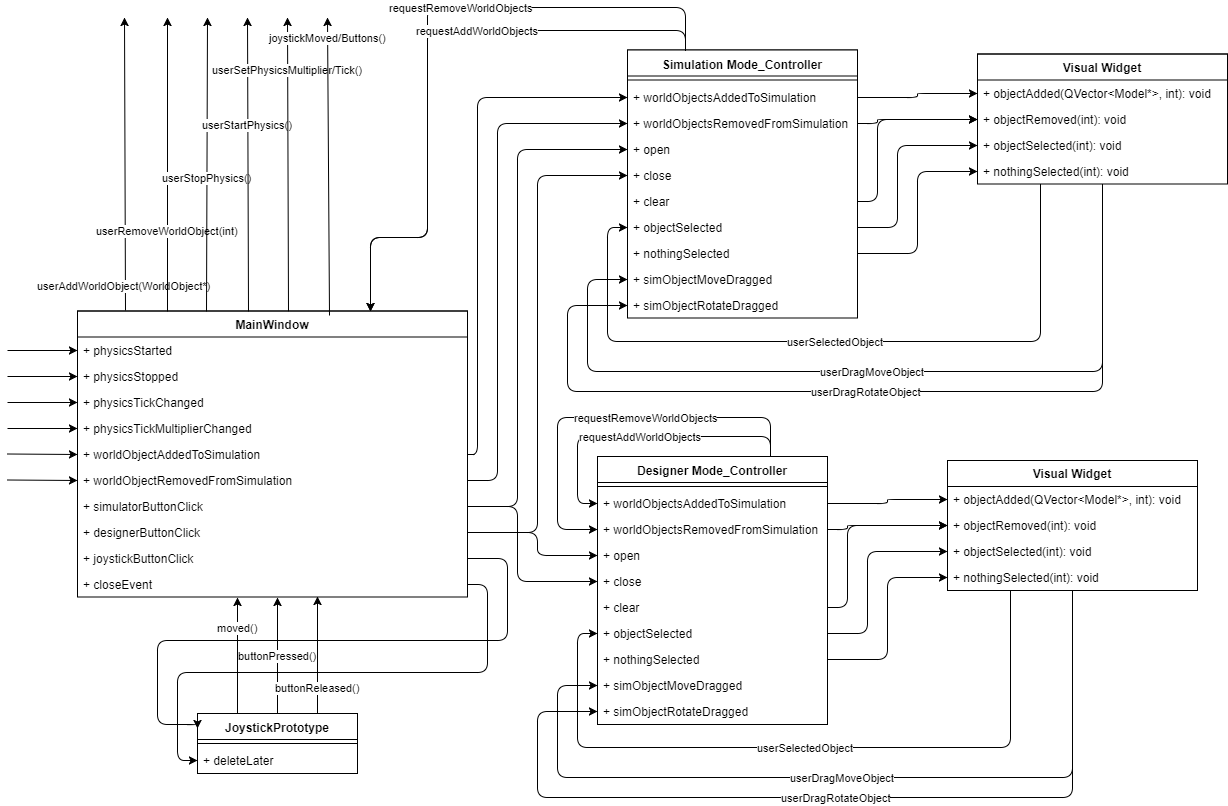
\includegraphics[scale=0.5]{./images_design/uml/DataFlow_UI}
 	\caption{Data flow of User Interface\label{uml:dataflow_ui}}
 	\end{center}
 \end{figure} 
 
 \subsubsection*{Layout}
  \begin{figure}[h!]
 	\begin{center}
 	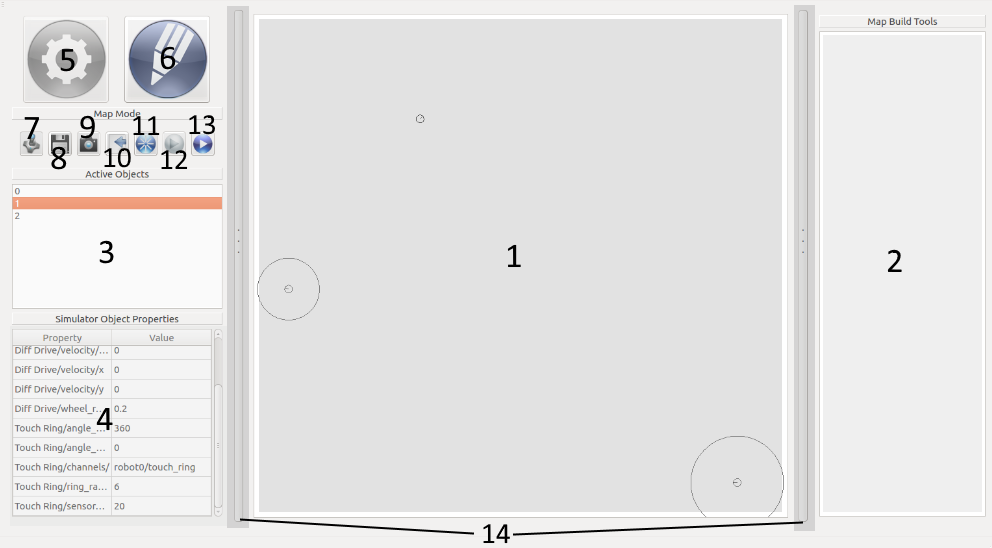
\includegraphics[width=\textwidth]{./images_design/UI_Overview}
 	\caption{Layout of the User Interface\label{fig:ui_overview}}
 	\end{center}
 \end{figure}
 
 Brief descriptions of the sections of the UI (Figure \ref{fig:ui_overview}).
 \begin{enumerate}
 	\item The World View widget\\
 	In Simulation Mode: Shows what's currently happening in the simulation\\
 	In Design Mode: Shows the world object that's currently being designed.
 	\item The toolbox\\
 	In Simulation Mode: Lists World Objects that have been loaded from file. They can be dragged into the simulation when it is not running.\\
 	In Design Mode: Shows the World Object Components which can be added to the World Object
 	\item Objects list\\
 	In Simulation Mode: Lists all World Objects currently in the simulation. They can be selected from this list.\\
 	In Design Mode: Lists all World Object Components currently on the World Object. They can also be selected from here.
 	\item Properties list\\
 	Both Modes: Displays and allows editing of whatever is currently selected
 	\item Simulation Mode button
 	\item Design Mode button
 	\item Opens a new joystick window
 	\item Saves the current simulation state
 	\item Takes a screenshot of the simulation
 	\item Opens a simulation, image (map), or world object file.
 	\item Time Warp
 	\item Resets the simulation
 	\item Starts/Pauses the simulation
 \end{enumerate}
 
 \subsubsection*{Design Details}
 \begin{itemize}
 	\item All events that affect the simulation backend (the physics or core) follow a circular data path. The UI generates an event and emits it $\rightarrow$ The affected object receives the event, acts on it, and sends a response $\rightarrow$ The UI receives that response and updates so the user knows what happened.
 	\item Object properties are shown through a Model-View controller. When an object is selected, its properties are loaded into the model and connected to the dataChanged signals it emits. When the user changes the data in the model, the property views read the new data and attempt to set it on the original Property object if the property is read-only.
 	\item The UI is constructed with a factory function for making the world view widget. This can be done because the widget follows a specific interface and allows for rewriting the world view without changing any of the rest of the application.
 	\item BUG: Currently, the user can change a read-only property on screen (this does not change the original property value, but the screen shows incorrect data)
 \end{itemize}
\subsection{World View}
\subsubsection*{Technologies Used}
\begin{itemize}
	\item Qt
	\item Qt Widgets
	\item Qt Graphics Framework
	\item Box2D
\end{itemize}
\subsubsection*{Overview}
The world viewer widget implemented in this project is called 'BasicViewer'. It uses the Qt Graphics Framework to create a 2D drawing canvas. The UML diagram for this class can be see in Figure \ref{uml:viewwidget}.

The UI can draw things on the widget by passing it a set of Models along with an integer reference. This reference could be the identifier of a World Object which the models represent, or it could be assigned by the UI. When the UI wants to change how this set of models is drawn, or remove them from the screen, this identifying value is used.
The options for how a shape is drawn include 'selected' or 'not selected', and 'solid', 'transparent', and 'not drawn'. Only one object (group of shapes with a single identifier) may be selected at a time.
 \begin{figure}
 	\begin{center}
 	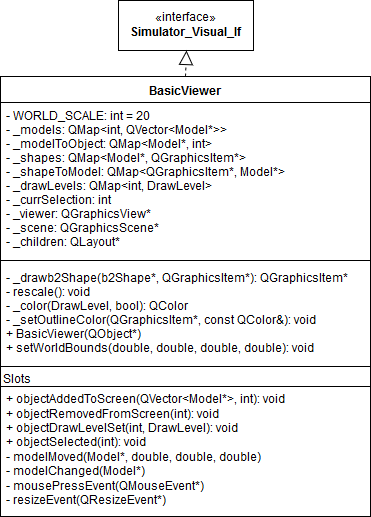
\includegraphics[scale=0.5]{./images_design/uml/BasicViewer}
 	\caption{UML of Visualization widget\label{uml:viewwidget}}
 	\end{center}
 \end{figure}
 
\subsubsection*{Design Details}
\begin{itemize}
	\item The viewer supports drawing any Box2D Shape type except for the b2ChainShape. 
	\item The widget contains both the QGraphicsScene and QGraphicsView internally. It lays out the QGraphicsView to fill itself completely on instantiation.
	\item The QGraphicsView::fitInView method appears to be broken in Qt 5.5, so the BasicView widget manually sets the viewport when it resizes.
	\item Rather than redraw an entire model when one of its children changes or moves, the widget connects to the signals of all the child models and just redraws the portions that change or move

\subsection{The main() Function}
\subsubsection*{Technologies Used}
\begin{itemize}
	\item Qt
	\item ROS
\end{itemize}

\subsubsection*{Overview}
The main() function serves a couple of important purposes.
\begin{enumerate}
	\item Create QApplication. This runs the event loop and represents the application as a whole.
	\item Call ros::spin() in a separate thread
	\item Connect the ros spin thread to the QApplication
	\item Load all valid plugins that can be found in \lstinline|../|
	\item Instantiate a system object for each interface
	\begin{itemize}
		\item ObjectFileHandler\_If
		\item Factory function for Simulator\_Visual\_If
		\item Simulator\_Physics\_If
		\item Simulator\_Ui\_If
	\end{itemize}
	\item Instantiate and start the Simulator Core
	\item Start the Qt Event Loop
\end{enumerate}

\subsubsection*{Design Details}
\begin{itemize}
	\item The ROS spin thread is connected to the QApplication for mutually assured destruction. If the ROS connection dies, then the application will close. If the Application closes, then the ROS connection will end. This prevents either from continuing in an invalid state without the other.
	\begin{lstlisting}
QFutureWatcher<void> rosThread;
rosThread.setFuture(QtConcurrent::run(&ros::spin));
QObject::connect(&rosThread, &QFutureWatcher<void>::finished, &app,
                 &QCoreApplication::quit);
QObject::connect(&app, &QCoreApplication::aboutToQuit,
                 [](){ros::shutdown();});
	\end{lstlisting}
	\item The directory above the executable is checked for plugins because that is, by default, where Catkin places shared libraries
\end{itemize}
\section{Plugins}
One of the main advantages to the design of this project is that it can be extended through WorldObjectComponent Plugins. Unfortunately, because it is a ROS package, the project (and any such plugins) must be built with Catkin and CMake. A number of plugins have been included with the project to provide much basic functionality, and those plugins can be used as examples of how plugins should be set up; however, not all plugins will follow the same patterns, so this section will describe the existing plugins as well as some of the requirements to build and use a plugin.
\subsection{Touch Sensor Ring}
The touch sensor ring plugin mimics a ring of touch sensors with a specific radius. It is intended to be used on circular robots, so that its radius can be set to the same as the robot. 
	The sensor ring can be set to sense a specific section of the circle, and the number of sensors used can be specified. Whenever the state of one of the buttons changes, a ROS message is published. Extra circles are drawn on the world visualization to show which touch sensors are triggered. An example of this can be seen in Figure \ref{fig:touchsensorexample}. Details of the properties exposed by the plugin and the ROS messages it utilizes can be found in tables \ref{tab:touch_ring_props} and \ref{tab:touch_ring_msgs}
	
	\begin{figure}[h]
		\centering
		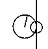
\includegraphics{./images_design/touch_sensor}
		\caption{Example of the touch sensor ring sensing something. The large circle is a robot, the small circle is the touched sensor point.}
		\label{fig:touchsensorexample}
	\end{figure}
\begin{table}[h!]
	\centering
	\caption{Properties exposed by the Touch Sensor Ring plugin}
	\label{tab:touch_ring_props}
	\begin{tabular}{c|c|c}
	Property Name & Data Type & Description\\ \hline \hline
	channels/output\_channel & String & The ROS topic to output sensor messages to\\ \hline
	angle\_start & Double (0-360) & Angle that the sensed section starts at\\ \hline
	angle\_end & Double (0-360) & Angle that the sensed section ends at\\ \hline
	ring\_radius & Double & Radius of the touch sensor ring\\ \hline
	sensor\_count & Integer & \makecell{Number of sensors spaced evenly in the slice\\ of the circle defined by angle\_start and angle\_end}
	\end{tabular}
\end{table}
\begin{table}[h!]
	\centering
	\caption{ROS Messages used by the Touch Sensor Ring Plugin}
	\label{tab:touch_ring_msgs}
	\begin{tabular}{c|c|c|c}
	ROS Topic & Message Type & In/Out & Description\\ \hline \hline
	channels/output\_channel & std\_msgs::ByteMultiArray & Out & \makecell{1-Dimensional vector with one\\ element for each touch sensor on\\ the ring. Untriggered buttons\\ are set to 0, triggered\\ ones are non-0.}
	\end{tabular}
\end{table}
\subsubsection*{Design Details}
\begin{itemize}
	\item All the required circle shapes for the touch sensors are generated at the start. They are added to and removed from the model when they become active or inactive.
	\item The touch sensor circle is a solid physics shape which can collide. This generates collision points from Box2D that can be used to know what is sensed.
	\item The body with the sensor ring fixture is held in place relative to the robot by a Box2D Weld Joint. The ring has a very low density (so as not to affect how the robot drives) so, due to the implementation of Weld Joints,  it is possible for the ring to behave in strange ways if it is larger than the robot it surrounds. Specifically, if there is a collsion and the robot continues to drive, the robot can be seen moving around within the touch sensor ring; it does not stay anchored in the center as one might expect.
\end{itemize}
\subsection{Custom Plugins}
Custom plugins should be ROS packages in the same workspace as the simulator package. The plugin's package.xml file should specify at least the following in order to resolve build order:
\begin{lstlisting}
<depend>sdsmt_simulator</depend>
<depend>sdsmt_simulator_box2d</depend>
\end{lstlisting}

Once Catkin is aware of package dependencies, the CMakeLists file must be set up to find the required libraries and files and build the plugin correctly.

First, there are a number of definitions and values that need to be set in order to compile and link the Qt-Specific portions of the plugin
\begin{lstlisting}
find_package(Qt5 REQUIRED COMPONENTS
  Core
)

set(CMAKE_INCLUDE_CURRENT_DIR ON)
set(CMAKE_AUTOMOC ON)

add_definitions(-DQT_PLUGIN)
add_definitions(-DQT_SHARED)

include_directories( ${CMAKE_BINARY_DIR} )
\end{lstlisting}

In order to resolve dependencies for Box2D and the header files from the simulator, find\_package needs to be called for the associated packages.
\begin{lstlisting}
find_package(catkin REQUIRED COMPONENTS
    sdsmt_simulator
    sdsmt_simulator_box2d)
    
catkin_package(
    CATKIN_DEPENDS
    sdsmt_simulator
    sdsmt_simulator_box2d
)
\end{lstlisting}


Finally, the plugin needs to be built as a shared library and linked against Qt Core libraries and the Box2D library.
\begin{lstlisting}
add_compile_options(-fPIC)

add_library([plugin name] SHARED ${CPP_SRCS} ${MOC_SRCS})
qt5_use_modules([plugin name] Core)

target_link_libraries(touch_sensor_plugin
  ${catkin_LIBRARIES}
)
\end{lstlisting}

The last detail is that the plugin must be deployed in the directory above the simulator executable. This happens by default when the simulator and plugin packages are in the same package and \lstinline|catkin_make| is used to build them. However, if they are in separate workspaces or one has been installed to a more permanent directory (either manually or with \lstinline|catkin_make install|) then extra care will need to be taken to ensure that this last requirement is met.

\subsubsection*{A Note About ROS Communications}
It is believed by the project team that, because the ros::spin() method was called from a thread other than the main one, all ROS message callbacks will be run from that thread. Care should be taken when defining callbacks in components to prevent race conditions which would result from this design. This issue was resolved in the Touch Sensor Ring plugin with the use of a Qt Signal and Slot. When a Qt Signal triggers a Slot of an object which resides in a different thread, the slot is queued for the second thread to receive naturally during its event loop, preventing any race conditions. The Touch Sensor Ring component has an internal signal and slot specifically for this purpose; the signal is emitted by the ROS callback function, and that copies the data from the callback into the main thread where it can be processed safely.

\end{itemize}  %% All tracks
% !TEX root = DesignDocument.tex


\chapter{System and Unit Testing Design}
This section describes the approach taken with regard to system and unit testing. It describes a number of specific tests and their results.  

\section{Overview}
The testing approach for this project is largely exploratory because the project is so graphically driven. These tests are basically comprised of simply observing the application after making changes, and determining whether or not those changes are reflected in the application.

There are also some unit tests for aspects of the project that can be tested algorithmically.

Much of our exploratory testing will be performed by beta users in the future.

\section{Test design and setup}
This section will describe how test cases were developed/designed, setup, and how they connect to the requirements.

\subsection{Application Window Opens Correctly}
Upon starting the program, a Qt window should open up in the foreground of the user's screen. This was tested through simple observation.

\subsection{Application Window Closes Correctly}
Upon clicking on the 'x' in the top right corner of the application window, it should be exited completely. This was tested through simple observation.

\subsection{User Interaction Generates Signals}
The user clicking buttons should generate signals which can cause events to be initiated by our code. In order to confirm that this works, slots were set up to listen to signals from the buttons which would cause visually obvious changes to occur within the application window. Then, these buttons were clicked, and it was confirmed that the correct changes happened.

\subsection{Application Window Resizes Correctly}
Resizing the window should be allowed, but should not cause graphical components to overlap, move outside the window, or shrink or grow to be unusually large or small on their x or y axis. This was tested by resizing the window first to be tall and thin, then short and thin, then short and wide, then tall and wide. It was confirmed that no unusual behaviors occured in any of these configurations.

\subsection{Robots Appear On Screen}
Each robot generated within the physics engine should also be visible within the simulation, assuming that the x and y coordinates of that robot are within the boundaries of the world view. To test this, a robot was generated at coordinates that should have put it in the center of the world view, and then it was confirmed that the world view now drew a circle at that location.

\subsection{Obstacles Appear On Screen}
Each obstacle generated within the physics engine should also be visible within the simulation, assuming that some part of the obstacle is within the boundaries of the world view. To test this, an obstacle was generated such that it was entirely within the world view, and then it was confirmed that the world view now drew the obstacle at that location.

\subsection{Application Receives Wheel Speeds}
The application should be able to receive wheel speeds from a seperate program, which it will use to apply forces to the robot within the physics simulation. To confirm that this work, we wrote a seperate Python application which publishes wheel velocities and observed our application using them to move a robot on the screen.

\subsection{Control Code Moves Robots}
Wheel speeds received from a separate program should move a robot in the active simulation accordingly. To test this, we set up the wheel speed generator to drive a robot in a figure-8. Then, with kinematic equations, these wheel speeds were converted to the velocity of the robot, which was handed to the physics simulation. The desired result was our simulated robot driving in a figure-8 after starting up the simulation. This was quite easy to evaluate visually.

This test was also run with the wheel speed generator outputting speeds to make the robot drive in a cricle, and again with speeds to make the robot drive back and forth along a line diagonally. Each drive pattern was observed working as intended.

\subsection{Collisions Function Correctly}
If a robot tries to move into or through another robot or an obstacle, it should fail to do so. Instead, it should stop just short, and its velocity in the direction of the thing it's colliding with should be set to zero, or it should push the thing it's colldigin with. Then, it can try again in the next time step. To test this, obstacles were set just inside each edge of the world view, so that the robot, spawned in the center of the world view would be boxed in. Then, the aforementioned figure-8 code was run and the robot was observed running into, but not entering each of the obstacles many, many times. 

In order to confirm that this would also work with other robots, three were all generated at different locations within the box of obstacles and were set to run with the same figure-8 control code. They were quickly observed colliding, and behaving in an acceptable manner.

\subsection{Multiple Robots Can Exists at Once}
Many robots should be able to exist at once, in different locations. To test this, three robots were loaded at different locations in the physics simulation, within the bounds of the world view, then it was confirmed that three circles appeared within the world view.

This fulfills the User Story contained in \ref{us:10}

\subsection{Changing Robot Properties in GUI Effects Simulation}
Changing the properties of a robot should have an immediate effect on the simulation. To test this, a property with a visually obvious result, specifically, the radius of the robot's touch sensor, was changed and it was observed that the size of touch sensor's indicator circle also changed.

\subsection{Touch Sensors Function Correctly}
Touch sensors should indicate when the robot they're attached to gets within a certain distance of another object in the world. To test this, a circle is being drawn to indicate a touch sensor. As the radius of the touch sensor is changed, the size of the circle can also be observed changing. Wherever an obstacle is detected by the touch sensor, it draws another much smaller circle along its radius. The robot was set to drive in a figure-8, and these circles were observed appearing and dissappearing as they should.

This contributes to the fulfillment of the User Story contained in \ref{us:7}

\subsection{Touch Sensors Publish ROS Messages}
Touch sensors should publish ROS messages to ROS tools whenever they're activated by a collision. This was tested by setting a robot with a touch sensor to drive in a figure-8 which was larger than the box of obstacles it was contained in. This caused many collisions, and therefore many touch sensor activations to occur. ROS messages were observed being generated properly by ROS tools.

\subsection{Selecting an Object in the Active Objects Menu Should Display the Properties of That Object}
When a row in the active objects menu that is not already highlighted is clicked by the user, it should become highlighted, and the properties being displayed in the Simulator Object Properties table should change to reflect the properties of the newly selected object. To test this, two robots with different touch sensor radius sizes were placed into the world, and it was observed that when the robots were switched between in the active objects menu, the touch sensor radius also changed in the simulator object properties table.

\subsection{When Switching Between Map and Designer Mode, the Map and Designer Mode Buttons Should Change Colors}
In map mode, the map mode button should be grey and the designer mode button should be blue. In designer mode, these colors should be swapped. To test this, the mode of operation switched back and forth from map mode to designer mode many times, and the colors were observed changing as intended.

\subsection{When Switching Between Map and Designer Mode, the Build Tools Should Change}
In map mode, the widget on the far right side of the screen should display map build tools, and in display mode, that widget should display designer build tools. To test this, the mode of operation was changed many times, and the widget was observed changing as intended.

\subsection{When Switching Between Map and Designer Mode, Available Buttons Should Change}
In map mode, there should be seven map design buttons below the mode of operation buttons, and in designer mode, there should be five designer buttons. To test this, the mode of operation was changed many times, and the buttons were observed changing as intended.

\subsection{Robot Designer Supports Multiple Body Shapes}
The user should be able to use the integrated robot designer to build robots with a number of body shapes, and to load them into the simulation. To test this, a robot was designed with a circular body, another with a rectangular body, and a third with an irregularly shaped body made up of connected polygons. Each was observed behaving as intended in the simulation while driving uninterrupted, and while colliding with other world objects.

This contributes to fulfillment of the User Story contained in \ref{us:3}

\subsection{Robot Designer Supports Multiple Drive Systems}
The user should be able to use the integrated robot designer to build robots with a number of drive systems, and to load them into the simulation. To test this, a robot was designed with differential drive and another with ackermann drive. Each was observed behaving as intended in the simulation while driving uninterrupted, and while colliding with other world objects.

This contributes to fulfillment of the User Story contained in \ref{us:3}

\subsection{Robot Designer Supports Multiple Sensors}
The user should be able to use the integrated robot designer to build robots with a number of sensors, and to load them into the simulation. To test this, a robot was designed with a lidar sensor and another with a touch sensor. Each was observed behaving as intended in the simulation while driving uninterrupted, and while colliding with other world objects.

This contributes to fulfillment of the User Story contained in \ref{us:3}

\subsection{Robot Designer Supports Any Number of Sensors on a Single Robot}
The user should be able to use the integrated robot designer to build robots with zero, one, or many sensors. Should they choose to put many sensors on a single robot, these sensors should be allowed to be of the same type, or differnet types. To test this, a robot was designed with no sensors, another with a single touch sensor, another with two lidar sensors, and another with one lidar and one touch sensor. Each was observed behaving as intended in the simulation while driving uninterrupted, and while colliding with other world objects. Each was also observed publishing messages as intended.

This contributes to fulfillment of the User Story contained in \ref{us:3}

\subsection{Integrated Joystick Tool Controls Robot}
The user should be able to use the integrated joystick tool to control a robot. To test this, the joystick tool was loaded up and connected to a robot, which was then controlled in the simulation by moving the joystick within the widget. Pushing the joystick towards the top of the widget was confirmed to cause the robot to move forwards, pushing the joystick towards the bottom was confirmed to make the robot move backwards, and pushing it towards either side was confirmed to make the robot turn left or right accordingly.

This fulfills the User Story contained in \ref{us:4}

\subsection{Drive System can be in Different Positions on Robot}
The user should be able to position a drive system wherever they want to on a robot. To test this, the robot designer was used to place a drive system in the middle of a robot, near the front of a different robot, and in the back left corner of another robot. Each was observed behaving as intended in the simulation while driving uninterrupted, and while colliding with other world objects.

This fulfills the User Story contained in \ref{us:5}

\subsection{Sensors can be in Different Positions on Robot}
The user should be able to position a sensor wherever they want to on a robot. To test this, the robot designer was used to place a sensor in the middle of a robot, near the front of a different robot, and to place one in the back left corner and back right corner of another robot. Each was observed behaving as intended in the simulation while driving uninterrupted, and while colliding with other world objects.

This fulfills the User Story contained in \ref{us:6}

\subsection{Lidar Sensors Visibly Detect Objects}
When an object is in range of a Lidar sensor, there should be a visual indication. This visual indication should be in the form of the lines representing the lidar sensor stopping short when they hit an object within their range. To test this, a robot with a lidar sensor was observed driving around many objects, and its sensor lines were observed shortening as intended while close enough to other objects.

This contributes to the fulfillment of the User Story contained in \ref{us:7}

\subsection{Images can be Imported as Maps}
The user should be able to load an image file as a map. This was tested by clicking the load map button and selecting an image file of a maze where all of the walls are completely black and everything else is completely white. The resulting map in the simulator was compared to the image, and confirmed to be very similar.

This contributes to the fulfillment of the User Story contained in \ref{us:9}

\subsection{User can Select Darkness Threshold for Image Map Importing}
The user should be able to select the darkness threshold for a map during the loading process. This should affect the objects created within the simulation. To test this, an image containing a rectangle that faded from completely white to completely black, surrounded by a white border on all sides was loaded at a threshold of 50, 100, 200, and 250. The size of the rectangle created in the simulation was observed to change accordingly.

This contributes to the fulfillment of the User Story contained in \ref{us:9}

\subsection{User can Select Size of Image Map in Simulator}
The user should be able to select the size of a map during the loading process. This was tested by loading the same image at different sizes and observing the objects loaded in the simulator to change sizes accordingly.

This contributes to the fulfillment of the User Story contained in \ref{us:9}

\subsection{Many Map Types can Be Loaded by Image Loader}
The map image loader should be able to load a wide variety of images as maps. This was tested by loading an image with rounded edges, an image with many colors in different shades, an image with concave shapes, and image with many seperate shapes, an image comprised of random noise, an entirely white image, and an entirely black image. Each was observed being loaded as expected.

This contributes to the fulfillment of the User Story contained in \ref{us:9}

\subsection{Maps can be Save and Loaded}
The user should be able to save and load maps as json files. These save states should include world objects, including robots and their properties. To test this, an image was loaded as a map, and two distinct robots were designed in the robot designer and placed into the simulation. The 'save map' button was clicked, and the json file format was selected. Then, a different image file was loaded as a map, two entirely different robots were designed and placed, and this too was saved. 

At this point, the first map was loaded by clicking the 'load map' button, selecting the json file format, and selecting the desired map. The simulation was observed getting set back to the state it had been in when the first map was saved. Robot objects and non-robot objects and all of their properties were maintained. Then the second map was loaded in the same way with the same results.

\subsection{Quicksave and Quickload Function Properly}
The user should be able to quicksave a simulator state, then, after making changes, return to that state with use of quickload. To test this, an image was loaded as a map, and two distinct robots were designed in the robot designer and placed into the simulation, then the quicksave button was clicked. Then, a different image file was loaded as a map, two entirely different robots were designed and placed.

Next, the quickload button was clicked and the simulation was observed getting set back to the state it had been in when the first map was saved. Robot objects and non-robot objects and all of their properties were maintained.

\section{Unit Testing}

\subsection{Dependencies}
We plan to use Catch unit testing framework for our unit testing. This only requires the inclusion of a single header and will be in the project; thus there are no outside dependencies.

\subsection{Writing and Running Tests}
Unit tests are included inside of the packages with the code that they test. The package \lstinline|pkg_CatchTesting| includes the Catch header file, a default Catch main source file, and a cmake file providing a macro to create Catch tests which can be run as part of the Ament build process.

\subsubsection*{Adding Tests}
Tests should be in their own C++ source file, which includes \lstinline|"Catch/catch.hpp"| which is available from the Catch Testing package. The source file should not define a \lstinline|main()| or invoke the Catch macro to create one; the file should contain only Catch tests.

Adding test files to the build is fairly simple, just copy the block in Listing \ref{lst:catchcmake} into the CMakeLists file for the package which the tests are for and modify it for the project. This block should be \textit{before} the \lstinline|ament_package()| function. Once tests are added to the build, they can be built and run using the command \lstinline|ament test|. This will run all unit tests and report whether they pass or fail. Unfortunately, the JUnit files exported by Catch are not compliant with GTest's modifications to the JUnit standard, so Ament will be unable to report which specific tests failed. Fortunately, the JUnit XML files can be found in \lstinline|[workspace root]\build\[package]\test_results\|; these files can be opened and read to determine which specific tests failed.

\begin{lstlisting}[caption={Example CMake code for adding a Catch test}, label={lst:catchcmake}]
if(BUILD_TESTING)
    find_package(sdsmt_simulator_catch_tests REQUIRED)

    ament_export_dependencies(
        sdsmt_simulator_catch_tests
    )

    # Hacky way to include the cmake file since (as far as I know) Ament does not provide a way to export
    # Other random files.
    set(CATCH_CMAKE "${sdsmt_simulator_catch_tests_INCLUDE_DIRS}/Catch/ament_cmake_add_catch_test.cmake")
    include(${CATCH_CMAKE})

    ament_add_catch_test(
        "[test name]"
        CPP_SOURCES [list of plain C++ sources]
        QT_SOURCES [list of C++ sources which need to be MOC'ed]
        QT_HEADERS [list of C++ headers which need to be MOC'ed]
        QT_LIBS [list of Qt Libraries to link against \{Core, Widgets, GUI, etc.\}]
        ROS_LIBS [list of other ROS package dependencies]
        LIBS [list of other libraries to link against]
        )

    # Example for building Model unit tests in the API package 
    # ament_add_catch_test(
    #     "model_datatype_tests"
    #     CPP_SOURCES tests/test_model.cpp
    #     QT_HEADERS include/sdsmt_simulator/model.h
    #     QT_LIBS Core
    #     ROS_LIBS "sdsmt_simulator_box2d"
    #     )
endif()
\end{lstlisting}

\subsection{List of Tests}
\subsubsection*{Tests for the Model class}
\begin{itemize}
    \item The Model transform is 0, 0, 0 on construction
    \item Using Model::setTransform changes the result of Model::getTransform correspondingly
    \item Setting Model transform results in Model::transformChanged being emitted
    \item Model shapes list is empty on construction
    \item Added shapes are reflected in calls to Model::shapes()
    \item Adding a shape multiple times does not create duplicates in Model::shapes()
    \item Removed shapes are reflected in calls to Model::shapes()
    \item Adding or removing one or more shapes results in Model::modelChanged being emitted (even if the shapes were added as duplicates or removed when they didn't exist)
    \item Model children list is empty on construction
    \item Added children are reflected in calls to Model::children()
    \item Adding a child multiple times does not create duplicates in Model::children()
    \item Removed children are reflected in calls to Model::children()
    \item Adding or removing one or more children results in Model::modelChanged being emitted (even if the models were added as duplicates or removed when they didn't exist)
    \item Calling Model::forceDraw results in Model::modelChanged being emitted
\end{itemize}
\subsubsection*{Tests for the Property class}
\begin{itemize}
    \item Testing of the static double\_validator function
    \item Testing of the static int\_validator function
    \item Testing of the static abs\_double\_validator function
    \item Testing of the static bool\_validator function
    \item Testing of the static angle\_validator function
    \item Property value can be set and retrieved with Property::set() and Property::get()
    \item Setting Property value results in emission of valueSet() in the Property and any PropertyValues observing it
    \item Requesting Property value from a PropertyView sets the value and results in emission of valueSet() in the Property and any PropertyValues observing it
    \item Requesting Property value from a PropertyView sets the value and results in emission of valueRequested() in the property
    \item Setting Property value can optionally emit valueRequested() in the Property
    \item PropertyValues can be copy-constructed to observe the same Property
    \item Deleting the Property observed by a PropertyView invalidates the PropertyView and does not cause nullptr dereferences
\end{itemize}  %% All tracks
% !TEX root = DesignDocument.tex


\chapter{Sprint Results and Prototypes}

This chapter discusses the results of each sprint and documents the evolving product. It covers the decisions and progress made in our 2D Robot Simulator during the first semester of our Senior Design class and is organized by Sprints, ranging from the zeroth sprint to the sixth.    

\section{Sprint 0 Report}
All work before Sept. 21st
\subsection{Sprint Backlog}

The backlog for the zeroth sprint consisted of choosing a physics engine, setting up all team members with Ubuntu version 16.04 and ROS, and examining the STDR 2D Robot Simulator for possible use. In sprint zero, we also decided to use Git and Trello for repositories and user stories.

\begin{itemize}
	\item Set up team members in Ubuntu environment
	\item Decide whether or not to use STDR simualtor
	\item Determine development tools 
\end{itemize}

\subsection{Deliverable}

The client initially requested that we alter the functionality of the existing 2D Robot Simulator called STDR. During sprint zero, however, the team established that it would be more effective to move toward the client's change requests by starting a new software entirely. The STDR was used for reference and to assist in setting up our architecture such that it would be more versatile and allow for future plug-ins.

\begin{itemize}
	\item Team research (MVP)
	\begin{itemize}
		\item Decision to start project from scratch rather than alter STDR simualtor
		\item Box2D as physics engine
		\item QT Creator as IDE
	\end{itemize}
	\item Environment setup
	\begin{itemize}
		\item Ubuntu v 16.04 
		\item ROS kinetic
	\end{itemize}
\end{itemize}

\subsection{Results of testing}

In this sprint, the team decided to use QT Creator as a development environment and Box2D as a physics engine, which we decided had enough options to get what our product needed without going overboard on physics capabilities we would never need to implement. The work load was partitioned into four parts, one for each team member, as the GUI, the world view, the physics, and the backend. The STDR was used for reference only, and team members moved forward with learning to use the tools for their partitioned sections of work.

\subsection{Successes and Failures}

Sprint zero was successful because by the end of it the team was structured, the work divided, and the environments set up such that code could be written in the preceeding sprint.

\subsection{Modifications Required}

As this was the first sprint, there were no modifications from previous sprint work or decisions. However, we veered from the initial client request to alter the STDR simulator, as we decided to start a new software from scratch which would implement the use of a physics engine and support future plug-ins.

\subsection{Sprint Review}

Sprint zero was a success in that we established Ubuntu 16.04 as an environment for our development, all team members installed necessary softwares like Qt Creator and ROS, and we met with the client to discuss software requirements.

\subsection{Sprint Retrospective}

In retrospect, the team felt very good about progress made during this sprint. We had planned to do research during the sprint, (on the STDR, architecture, IDE, physics engine, and world view widget), and by the end of the sprint we had enough user stories and information to start writing code. Therefore we exceeded our sprint zero goals and promptly set the product in motion.


\section{Sprint 1 Report}
Sept. 21st - Oct. 5th
\subsection{Sprint Backlog}

The goals for this sprint included establishing a backlog. Some examples of user stories are supporting multiple robot shapes, being able to build robots from the program, and considering physics options like sticky wheels and moving map objects. These early user stories drove the creation of wireframes in this sprint, and ultimately the choices of the architecture design and tools used.

\begin{itemize}
	\item Create backlog of user stories
	\item Create UI wireframes
	\item Begin structuring architectural layers
\end{itemize}

\subsection{Deliverable}

At our first couple of client meetings, we discussed uses and overview of the product and delivered wireframes for a product GUI as well as a world view QT widget using Qt Graphics Framework. We also had a physics demonstration which printed out vector coordinates of two objects colliding using Box2D, and one team member determined how to use Catkin to build a Qt Widgets project. It was also during this sprint that we created our software contract. The deliverables were those wireframes, examples,the contract, and a Trello backlog of user stories.

\begin{itemize}
	\item Team research applications (MVP)
	\begin{itemize}
		\item Clickable UI
		\item Physics simulation example
		\item Catkin build functionality
	\end{itemize}
	\item Tools and documentation
	\begin{itemize}
		\item First draft of software contract
		\item Trello backlog of user stories
	\end{itemize}
\end{itemize}

\subsection{Results of testing}

Testing in this sprint was indepenedent among team members: the physics member tested uses and limits of Box2D, the UI member created a clickable UI, the world view member created a QT widget, and the backend member utilized Catkin to develop an easy way to run the project. The client accepted our software contract and approved both the cliackable UI and user stories.

\subsection{Successes and Failures}

We met the sprint one goals by the end of our two-week sprint. We established a backlog of user stories on Trello and all team members created GUI wireframes which were later used to make an initial clickable GUI and ultimately an MVP in sprint four. By the end of the sprint, the work was partitioned and the beginnings of a layered software architecture had been established.

\subsection{Modifications Required}

There was little modification from the zeroth sprint to the first, except to clear up misunderstandings about specific uses of the software. For example, it was unclear during the previous sprint whether a running simulation should pause when prompted, or reset entirely. We reached the conclusion that Qt Graphics Framework should be used for the world view widget, rather than the OpenGL widget we originally planned for. The main uses remained the same.

\subsection{Sprint Review}

Sprint one was a success in that we had a compilable project by the end of it. The four wireframes produced during the sprint were discussed with the client and we decided to take a single-window approach rather than a multi-window approach. This approach was intended to make the simulator feel like a game design engine, which was deemed desirable because the main users of the application would likely be familiar with game design applications. We established a backlog based on requests given in client meetings and all team members wrote code which applied to their section of work and would ultimately become part of the MVP.

\subsection{Sprint Retrospective}

In retrospect, the team felt okay about progress made during this sprint. We had planned to have a solid round of deliverables, which we did. We established a first draft of an architecture for the software and completed our software contract without issues. The team felt that the product was moving more slowly than planned, but that that would change once an MVP was produced. We may have lacked a little in communication due to the work being clearly divided, but bi-weekly team meetings held the project's best interests together.


\section{Sprint 2 Report}
Oct. 5th - Oct. 19
\subsection{Sprint Backlog}

The backlog for sprint two was to create a minimum viable product. This goal involved finishing interfaces, integrating the world view into the UI, and spawning a robot in the world view. The product was to be written in QT Creator such as to include a tab-like design with a simulator, a robot designer, and a map designer. The spawned robot necessary for the MVP was to be run via a python script to loop in a figure-8.

\begin{itemize}
	\item Create MVP
	\item Create interfaces for partition communication
\end{itemize}

\subsection{Deliverable}

Our major deliverable for this sprint was the MVP, which we showed to the client in a demo where we ran the single spawned robot on the figure-8 python script. To accomplish this, we had some minor deliverables like finishing interfaces for the UI and physics engine, and integrating the world view with the UI menus. The robot spawned in the middle of the world view and its velocity could be directly controlled with the python script.

\begin{itemize}
	\item Minimum Viable Product (MVP)
	\begin{itemize}
		\item Spawn single robot in center of world view
		\item Robot moves via python figure-8 script
		\item Finish interfaces for physics engine
		\item Finish interfaces for UI
		\item Integrate world view widget with UI
	\end{itemize}
\end{itemize}

\subsection{Results of testing}

Testing for this sprint was "as viewed" by the team members. The UI designer tested clickability of buttons and display of neccessary menus. The physics member tested a numerical output of two objects colliding. The backend member tested the MVP with the figure-8 python script and spawning of a single robot. During this sprint, we established that our product would, for the most part, have to be tested by users. Much of the code would not be able to be unit tested due to it being UI code or having infinite input parameter options.

\subsection{Successes and Failures}

In this sprint we succeeded in producing an MVP. We  established interfaces which would later be used to communicate via slots and signals between the UI, the world view, and the physics simulator. The single robot which spawned in the center of the world view could only spawn in the center and was hard-coded to spawn once. 

\subsection{Modifications Required}

There were no modifications from the first sprint to the second because the team was focused on producing an MVP. The client was pleased with said MVP, and no requests for change were made.

\subsection{Sprint Review}

Sprint two was a success in that we produced an MVP able to simulate a single robot on the clickable UI. Though it was hard-coded and our list of deliverables was small, this paved the way for future development. The client was very pleased with our progress and pushed to move toward sprint three goals of robot rotational capabilities and the option to spawn robots in locations other than the center of the world view.

\subsection{Sprint Retrospective}

In retrospect, the team felt substantial progress was made during this sprint. We produced an MVP and had the interfaces necessary to begin setting up communication between the UI, world view, backend, and physics simulator.


\section{Sprint 3 Report}
Oct. 19th - Nov. 2nd
\subsection{Sprint Backlog}

The backlog for this sprint involved enhancing the MVP and creating our first client presentation. The MVP allowed for the spawning of a single robot in the center of the world view, so a goal in this sprint was to spawn multiple robots at random orientations and in random locations across the map. We also wanted to be able to display properties for these robots, and select and change the properties displayed.

\begin{itemize}
	\item Allow for robots spawning at non-center of map
	\item Allow for robots to rotate while moving
	\item Be able to display and change robot properties
	\item Find a way to pass shapes around threads
\end{itemize}

\subsection{Deliverable}

The deliverable for this sprint was a prototype consisting of three robots which spawned at random locations in various orientations and moved in giant figure-8's across the world view. This was paired with the addition of viewing robot properties for one of the robots. The spawned robots were hard-coded. The progress was shown as a demo in a client meeting.

\begin{itemize}
	\item Demo of new features
	\begin{itemize}
		\item Multiple robots spawning randomly on map with random orientation
		\item Robots using differential drive kinematics
		\item Python script to drive differential drive robots in figure 8
		\item Being able to see and modify properties of robot (velocity, differential drive parameters...)
	\end{itemize}
\end{itemize}

\subsection{Results of testing}
During this sprint, we made a major architectural decision based on experimentation with integrating Box2D and threads. It was determined that continuing the multi-threaded architecture would be difficult and result in many future bugs. 

\begin{itemize}
	\item Decision was made to abandon multi-threaded design.
	\begin{itemize}
		\item Box2D does not play nicely with multiple threads
		\item It is ok if the simulation lags due to all computation in one thread because eventually timestamps will be published and control code will use that rather than its own internal clock
	\end{itemize}
\end{itemize}

\subsection{Successes and Failures}

In this sprint we succeeded in improving the MVP. We were able to show the client a product where three robots spawned in random locations with random orientations and moved about the world view, sometimes collided. We failed to implement a goal of making those robots selectable such that a specific robot's properties could be set.

\subsection{Modifications Required}

There was an architectural modification in this sprint: the switch from multi-threading to a single thread. This was known to have the potential for a slower program but we justified it with ease of code and lack of bugs. We expected the lag would be a minor issue.

\subsection{Sprint Review}
Our first team presentation was successful. The client was happy with the prototypes of our MVP and improved MVP. The team felt that good progress was made and despite the delay of switching from multi-threading to a single thread, we were able to get back on track and ready for sprint four.

\subsection{Sprint Retrospective}
In retrospect, there was no way to know without applying the project that the original multi-threaded approach wasn't going to work out. Luckily we came to this conclusion in sprint three with plenty of time to correct the architecture. Everything else in this sprint went smoothly, team coding sessions emerged as a form of integrating project partitions and proved successful.

\section{Sprint 4 Report}
Nov. 2nd - Nov. 16th
\subsection{Sprint Backlog}

The backlog for this sprint included allowing selection of robots from the world view and a side menu in the UI, implementing LIDAR and touch sensor plugins, loading of obstacle (map) files, and a prototype joystick for the UI. We also had to decide on a direction for the physics aspect of the project because the MVP involved a hard-coded robot a with specific design and we were ready to start looking at alternate robot possibilities.

\begin{itemize}
	\item Decide between kinematics and full-simulation physics
	\item Allow selection of robot from main view and UI menu
	\item Prototype joystick UI
	\item LIDAR plugin
	\item Touch sensor plugin
	\item Load obstacle files
\end{itemize}

\subsection{Deliverable}

In sprint four, we delivered the ability to select a robot from a menu in the UI and load obstacle files. The touch sensor implementation plus an obstacle file of four squares emulating a "room" assisted in confirming the correct response from collisions. We presented the physics decision to move away from the hard-coded differential drive and the client informed us of some possible changes.

\begin{itemize}
	\item Demo of new features
	\begin{itemize}
		\item Physics decision
		\item Ability to select a robot from a UI menu
		\item Ability to load obstacle files
		\item Confirmed collisions
		\item Touch sensor implementation
	\end{itemize}
\end{itemize}

\subsection{Results of testing}

In this sprint, we decided to change a few things in the project in order to reach an outcome as versatile as possible. After implementing the differential drive with collisions, we decided to rip, root, and reboot the physics aspect of the project. Loading the obstacle files required use of some of the interfaces created in sprint one.

\subsection{Successes and Failures}

Touch sensors and obstacles took longer than expected to implement and required major changes in object interfaces. As a result, the ability to select a robot by clicking its image was delayed and the LIDAR plugin was not written. The joystick prototype was not completed. The client also mentioned ROS 2 as a possible target in developing this project.

\subsection{Modifications Required}

While the touch sensor plugin was being written, it was discovered that Box2D can be leveraged to model a top-down vehicle. As a result, it was decided that this method of modeling robots should be used instead of kinematic modeling. The original robots spawned in the sprint two and three demos used a kinematic differential drive. The client warned us to watch out for possible changes from ROS to ROS 2 and we also discussed changing the foundation of differentiating between map objects and robots. We decided the product would be more useful if robots and map objects were created and treated the same way. Thus, we set out to redo the UI such that "Simulation Mode" would become a "Simulator" while "Map Mode" and "Robot Mode" would merge to become a single "Designer". This would allow for the creation of non-static map objects such as moving doors and doors with sensors. Overall, this would make the software more versatile.

\subsection{Sprint Review}

The client was again pleased with progress made. Our next target features were identified as implementing obstacles and some sort of sensor equipment so that the application could potentially be used in a class project. This along with revamping the UI, fixing the hard-coded kinematic physics, and implementing the Designer for world view objects led the direction we took moving into sprint five.

\subsection{Sprint Retrospective}

In retrospect, sprint four was pivotal as a post-MVP turning point for the product. We had enough code written to determine what was working and what was not, and made decisions that would ultimately push the product to be as versatile as possible.


\section{Sprint 5 Report}
Nov. 16th - Nov. 30th
\subsection{Sprint Backlog}

The backlog for this sprint included no programming. It was a sprint of documentation, client presentation number two, a discussion on ethics, and team evaluations.

\begin{itemize}
	\item Documentation
	\begin{itemize}
		\item Overview
		\item Project Plan
		\item Requirements
		\item Design
		\item Test Plan
		\item Prototypes
		\item Software Contract	
	\end{itemize}
	\item Presentation
	\item Ethics Quiz
	\item Team Evaluations
\end{itemize}

\subsection{Deliverable}

In sprint five, we focused on documentation catch-up. We wrote most of this document during sprint five, as well as our second client presentation, our team evaluations, and completeing a quiz on ethics in computer science.

\begin{itemize}
	\item Client presentation showcasing:
	\begin{itemize}
		\item Changes since STDR
		\item New GUI
		\item Physics decisions
		\item Future sensor implementation plans
	\end{itemize}
	\item Team evaluations
	\item Senior Design Final Documentation
	\item Ethics discussion
\end{itemize}

\subsection{Results of testing}

Our presentation was well-recieved by the audience and client alike. We decided to split up the documentation as much as possible such that the team members each wrote about sections of code they had written or architectural decisions they had made. We decided to include a side by side comparison in our presentation of our software against the STDR. This video was more effective to show differences than a dotted list would have been.

\subsection{Successes and Failures}

Our presentation was a success. The audience understood the project and we had ample imagery to show the changes we had made. We succeeded in submitting our team evaluations on time and bonded over a long discussion about the ACM code of ethics. We procrastinated a bit on the documentation but in the end, it got completed. 

\subsection{Modifications Required}

There were no major changes made during this sprint, except to shift the team's focus from coding to documentation. We had a lot of changes to make to the documentation, as we previously hadn't had all the information necessary to fill out several sections.

\subsection{Sprint Review}

The team felt that this sprint was successful despite writing no code and looking at the software itself very little. It was used mostly for reference to complete the documentation. We were able to complete all backlog items for this sprint and set up team members' tasks for the winter break.

\subsection{Sprint Retrospective}

In retrospect, sprint five was necessary and felt rushed. Writing documentation is, of course, less enjoyable than writing a 2D robot simulator and therefore we lacked some of the passion we had as a team for the previous five sprints (0-4). The ethics discussion really helped to give us all a sense of each other's priorities when it comes to developing software. Even though our software does not posess much controversy when it comes to ethics, understanding each other as individuals assisted in building a strong team connection.


\section{Sprint 6 Report}
Nov. 30th - Jan. 11th
\subsection{Sprint Backlog}

The entire Christmas break was designated to this sprint. The backlog for this sprint included fnishing the prototype joystick for the UI, adding Doxygen to the code, implementing image loading for the map, redoing the physics, loading and saving objects, LIDAR and possibly other sensors, time warping the simulation, and more documentation.

\begin{itemize}
	\item Joystick Prototype
	\item Doxygen	
	\item Image Loading
	\item New Physics
	\item Object load/save
	\item LIDAR
	\item Maybe other easy sensors
	\item Time Warp
	\item Full Spring Semester Plan Draft
\end{itemize}

\subsection{Deliverable}

In sprint six, we started a lot of features that did not get fully implemented, such as the joystick, image loading, and loading and saving world objects. User stories completed were the LIDAR and determining a plan for the remaining spring semester sprints.

\begin{itemize}
	\item New Physics
	\item Spring Semester Plan
	\item LIDAR sensor
\end{itemize}

\subsection{Results of testing}

At this point we determined our software was pretty functional in terms of the original goal. We compiled a list of new features left to implement before we started testing and collecting bugs. This list included more sensor plugins, more component plugins, the joystick control, world object designer, and saving/loading files.

\subsection{Successes and Failures}

This sprint, while slow, was successful as far as creating a plan for what remained of the project. We determined the software could not be tested by the spring semester robotics class but we would be able to write some tests for specific features. Image loading ended up being a more difficult task than anticipated due the need to break large image bodies into Box2D-compatible shapes.

\subsection{Modifications Required}

A couple decisions were made during this sprint, such as choosing not to try and test our software with the spring robotics class and also altering the physics. Some of the tasks were re-assigned and we decided on most important features to implement during the following semester.

\subsection{Sprint Review}

This sprint was successful as a planning sprint. We made a couple design decisions, worked with the client to compile a list of desired features moving forward, and assigned tasks to team members.

\subsection{Sprint Retrospective}

In retrospect, sprint six was a lax sprint that set the framework for the sprints to come. The team didn't communicate much over the break, though that was expected. Overall, it was a necessary sprint that solidified our plans for the future.

\section{Sprint 7 Report}
Jan. 11th - Jan. 25th
\subsection{Sprint Backlog}

The backlog for this sprint included finishing the joystick prototype, finishing the image loading, testing the software on Windows and ROS2, and implementing differential drive and the circle plugin.

\begin{itemize}
	\item Joystick Prototype
	\item Run on Windows
	\item Image Loading
	\item Differential Drive
	\item Circle Plugin
	\item Test with ROS2
	\item Load / Save files
\end{itemize}

\subsection{Deliverable}

In sprint seven, we focused on finishing some of the user stories started in sprint six, as well as implementing some new plugins and testing our product with different environment variables. The joystick prototype was completed and good progress was made in the realm of image loading.

\begin{itemize}
	\item Bug Fixes:
	\begin{itemize}
		\item Robot selection in active list matching green robot
		\item Properties updating when changed
		\item No NaN at start bug
		\item No crash while coloring shapes	
	\end{itemize}
	\item Project builds with ROS2
	\item Project works on Windows 10
	\item Moveable joystick window
\end{itemize}

\subsection{Results of testing}

Our product worked with ROS2 and also on Windows 10, but only for specific team members. One team member could not get the product to run on his Windows 10 despite seemingly no difference from the environment used by other team members. We discussed trying the product out on Mac OS as well, but could not find a viable machine on which to test it. It was in this sprint that we really started collecting and fixing bugs, because we finally had enough of a product to determine what was and was not working. 

\subsection{Successes and Failures}

We successfully adapted our project to run on Windows 10 and with ROS2, expanding our deployable environment requirements from strictly Unix systems, though we were not able to test it on Mac OS. Loading images as well as loading and saving files were pushed to backlog for the next sprint. The joystick was completed but not yet integrated into the software. Some bugs that hindered development were fixed.

\subsection{Modifications Required}

While there were no changes to the product architecture in this sprint, we did add in support for ROS2 and Windows 10. We had a few iterations of algorithms before solidifying a method for image triangulation. A few bugs popped up that required fixing, but they were promptly taken care of.

\subsection{Sprint Review}

The team felt that this sprint was successful because we established product compatibility with Windows 10 and ROS2. We lacked a little on implementation of new features but made headway with the joystick control and image loader as well as a couple client-requested plugins.

\subsection{Sprint Retrospective}

In retrospect, progress was slow during sprint seven as far as product development but we made good progress in expanding our client options with testing on Windows 10 and using ROS2. This will ultimately make our product more desireable in the testing and usage phases to come after this semester ends.


\section{Sprint 8 Report}
Jan. 25th - Feb. 8th
\subsection{Sprint Backlog}

The backlog for this sprint included completeing the image loading, integrating the joystick control, and implementing rectangle and ackermann steer plugins.

\begin{itemize}
	\item Image Loading
	\item Implement Ackermann steering
	\item Rectangle plugin
	\item Integrate joystick
	\item Control script for joystick
\end{itemize}

\subsection{Deliverable}

In sprint eight, we finished the image loading functionality, ackermann steering, the rectangle plugin, and controls for the joystick, which got integrated into the software. We did some backend clean-up as well that was not necessarily visible at the product frontend but left nicer source code for future developers.

\begin{itemize}
	\item Boilerplate start for image loader
	\item Simple Shape plugin
	\item UI bug to resize screen
	\item DLL fixes
	\item Clone function for world objects
	\item Joystick integrated with signals to physics models
	\item Lidar sensor
	\item Update Box2D version
	\item Rectangular robot
	\item Ackermann steering
	\item Consolidate packages for product
\end{itemize}

\subsection{Results of testing}

The joystick did not integrate as smoothly as planned, and some alterations had to be made in order to prevent a memory leak in the program. Rectangular robots and Ackermann steering both worked as planned except for the appearance of the "jello" effect, whereby the way Box2D handles welded objects made a particular robot wobble uncontrollably while moving.

\subsection{Successes and Failures}

We successfully integrated the joystick and implemented both rectangle and Ackermann plugins for the software. There was some bug fixes and code clean-up that went smoothly, such as new functions for world objects needed by the designer and enabling a logical user resize of the window. A couple issues we ran into were a minor memory leak that was fixed and the robot "jello" effect which prompted us to build in a window where users can alter robot mass settings until it no longer wobbles. The client would have preferred if the software could handle this but we decided to give default mass settings and otherwise keep it open-ended in case different users have different requirements for the individual simulations.

\subsection{Modifications Required}

Interaction between Box2D and world objects created the issue of wobbling wheels or the "jello" effect, which will have to be dealt with by users in the future via altering object mass until the desired effect is achieved. The UI was modularized by creating the mode controller object, such that the designer and simulator were controlled as mode controller objects by the main UI. This cleaned up the UI code and minimized code repetition which was getting imense with the creation of the world object and simulation designers. Other backend cleanup was implemented as well, such as DLL alterations and updating the version of our Box2D library.

\subsection{Sprint Review}

The team felt that this sprint was successful because we integrated the joystick, implemented rectangular robots and Ackermann steering, and continued to make progress with the image loader. We were happy to see that progress didn't slow too much with the transition into spring semester and we were still making strong headway with the product.

\subsection{Sprint Retrospective}

In retrospect, sprint eight took some of the pieces the team had been working on in previous sprints and brought them together. We successfully completed implementation of the joystick and the rectangle and Ackermann plugins. We came upon the issue of the "jello" effect, which we discussed with the client in later sprints to determine that it will be an ongoing issue with the software that individual users will have to play around with to obtain desired effects.

\section{Sprint 9 Report}
Feb. 8th - Feb. 22nd
\subsection{Sprint Backlog}

The backlog for this sprint included integrating the image loader, implementing the robot designer, starting a user manual, and fixing bugs that popped up during development in the previous sprints.

\begin{itemize}
	\item User Manual Documentation
	\item Integrate image loading
	\item Object Designer	
	\item Fix Joystick bugs
	\item Fix Ackermann Steer bugs
\end{itemize}

\subsection{Deliverable}

In sprint nine, we accomplished some bug fixes and integrated the image loader such that the user could choose any image, select a greyscale number, and import it into the simulation as a series of Box2D triangles. We also started discussing the user manual and things to include.

\begin{itemize}
	\item Bugs Fixed:	
	\begin{itemize}
		\item Joystick key selection
		\item Joystick sending correct numbers
		\item Ackermann steering glitch
	\end{itemize}
	\item Image loading with triangulation integrated into product
	\item Picked environment for User Manual
\end{itemize}

\subsection{Results of testing}
We found some bugs in the josytick and Ackermann steering because of our testing in this sprint, which were quickly resolved. The client decided he would like us to use Sphinx for the user manual with possible future implementation in the Senior Design class to replace LaTex.

\subsection{Successes and Failures}
Some of our implemented features required bug resolutions in this sprint, like the joystick and Ackermann steering. Map import button worked, but the images did not scale correctly. The object designer was not completed.

\subsection{Modifications Required}

In this sprint, we picked an environment for writing the user manual and integrated the image loader, which responded interestingly to some of the testing images. Because some of the images contained very curved lines and some contained very thin lines, we decided to allow the user to define a few settings that would determing how "precise" they needed the image to be once loaded into Box2D-compatible triangles. Other than that, the World Object Properties Wrapper was updated to work for both objects and components. This was necessary for modularity between the designer and the simulator when adding components to the tools lists.

\subsection{Sprint Review}

The team felt that this sprint was successful because we integrated the image loader, which the client was very pleased with, and made modifications necessary to implement the world object designer. We also started the user manual, which didn't really need to be completed until future sprints, so we felt we were still progressing with strong momentum.

\subsection{Sprint Retrospective}

In retrospect, sprint nine displayed our dwindling reservoir of new features to implement. At this point, it was basically the designer and some plugins that we had left before testing, documentation, and bug collecting would completely take over our time.

\section{Sprint 10 Report}
Feb. 22nd - Mar. 8th
\subsection{Sprint Backlog}

The backlog for this sprint included completing the world object designer, implementing file load/save, enabling the movement and rotation of objects in the world view, and fixing bugs.

\begin{itemize}
	\item Object Designer
	\item Time warping / speed button
	\item File Load / Save
	\item Rotate and Move World Objects
	\item Fix Image Loader bugs
\end{itemize}

\subsection{Deliverable}
In sprint ten, we confirmed functinoality of plugin loading, implemented rotating/moving world view objects, and worked on, but did not complete, the object designer. We also globalized World Object Component to make objects moveable on the map and fixed bugs like the program crashing while loading many world objects, objects being moveable during simulation play, lidar seeing invisible or non-colliding objects. We also got the speed button functioning just in time for the client presentation next sprint.
 
\begin{itemize}
	\item Fixed LIDAR bugs	
	\item Speed Button
	\item Added Rotate and Move World Object Tools
	\item Fix Image Loader bugs
	\item Changed Property to have distinct incoming/outgoing signals
	\item Able to build shape, sensor plugins
\end{itemize}

\subsection{Results of testing}

We were able to test the planned functionality for plugin components, which worked. The object designer worked after some modification, and we were able to export built robots to the simulator. Objects on the world view rotated and moved correctly for the most part, with some minor bugs in the designer using the rotate tool. We had to alter the signals for world object properties to the UI in order to get them updating in the backend models.

\subsection{Successes and Failures}
We successfully tested our component plugin compatibility. We also were able to fix some bugs with the lidar and image loader, and alter the properties signals to incorporate user changes in the models. During this sprint, our scrum master had to reimage his computer, which took a chunk of time out of his sprint schedule. The world object designer from the backlog did not get completed. However, we still completed most of the backlog items and made good progress in the product.

\subsection{Modifications Required}
We had to make world objects global in order to successfully get them to move on the world view. We also cleaned the makefile and debug/release flags, added epsilon checking for property values closer to 0. For the time warping, we modified the base speed of the simulation to be slower. This allowed us two levels of "faster" simulation without producing a glitchy output.

\subsection{Sprint Review}
The team felt that this sprint was successful despite the reimaging of a laptop. We were able to piece together some of the final user stories that we planned to get done before our final client presentation. Aside from the incompletion of the world object designer, which was pushed onto the next sprint.

\subsection{Sprint Retrospective}

In retrospect, sprint ten was a good preparatory sprint for the final client presentation. Much of what we got done was easy to show in a demo and thus created a more significant effect when we later showcased the progress we had made on the project.


\section{Sprint 11 Report}
Mar. 8th - Mar. 22th
\subsection{Sprint Backlog}

The backlog for this sprint included file load/save, JSON file formatting, client presentation three, integrating the world object designer, and some documentation.

\begin{itemize}
	\item Establish JSON file format
	\item Load / Save JSON files	
	\item Client Presentation showcasing:
	\begin{itemize}
		\item Named the product (finally) 
		\item Custom positioning of wheels and sensors
		\item Image Loading	
		\item Multiple drive systems
		\item Multiple sensors
		\item Various robot shapes (rectangular)
		\item Built in joystick control
	\end{itemize}
	\item Integrate Object Designer
	\item Remaining Documentation	
	\begin{itemize}
		\item Testing
		\item UI
		\item Sprints and Prototypes
		\item User Manual
	\end{itemize}
\end{itemize}

\subsection{Deliverable}
In sprint eleven, we completed the world object designer, completed simulation save/load, established our file format for world objects, divied out the remaining Documentation work, and gave our third client presentation.

\begin{itemize}
	\item World Object Designer
	\item World simulation loading
	\item Removed QSharedPointer requirement from file loader returns
	\item Client Presentation III
	\item Divided remaining Documentation work
	\item Established JSON file format and began work on load / save
\end{itemize} 


\subsection{Results of testing}
We got the designer fully integrated, added names to active objects list, altered plugin model sizes so they can be drawn in designer widgets, enabled modification of properties in the designer. To accomplish these, we had to remove the QSharedPointer requirement from file loader returns. We decided to go with a video demo for our presentation, rather than a live demo, and used the same presentation layout as with previous client presentations.

\subsection{Successes and Failures}

Our presentation was successful. The client and class were pleased with our progress and we were finally able to show some variation in the robots we were simulating, like a rectanglular robot with Ackermann steering. We successfully integrated the world object designer, although not in time to include it in the presentation. Some of the save/load operations we were working on also did not get implemented in time for the presentation.

\subsection{Modifications Required}
We had no major modifications during this sprint, aside from removing QSharedPointers and deciding on a file format for world objects. The object designer was finally integrated so a few bugs popped up with that, which didn't get fixed until sprint twelve.

\subsection{Sprint Review}
The team felt that this sprint was successful. We gave a good presentation, other than the fact that our lack of testing reflected poorly, and continued to make progress with the final product features. The client was happy with our work and we were almost at a point of completely switching over from development to bugs and documentation.

\subsection{Sprint Retrospective}

In retrospect, sprint eleven was where our early design decisions for flexibility and expansion really started to show. We were able to create plugins for some demo robots and actually use them in the simulation. We also gave a good final presentation to showcase this and successfully finished the last major development feature: the world object designer.


\section{Sprint 12 Report}
Mar. 22th - Apr. 5th
\subsection{Sprint Backlog}

The backlog for this sprint included fixing bugs, implementing quick save/quick load, documentation, design fair poster board, and finishing up the load/save file operations.

\begin{itemize}
	\item Fix UI Bugs
	\begin{itemize}
		\item Name and Type prompt for exported robots
		\item Black borders around tool widgets
		\item Icon Reselections
	\end{itemize}
	\item Quick Save/ Quick Load
	\item Load / Save World Object Buttons
	\item Load / Save Simulation Buttons
	\item Documentation
	\item Design Fair Preparations
\end{itemize}

\subsection{Deliverable}
In sprint twelve, we fixed some glaring bugs, changed the icons to all fall under one license, created some example robot files, implemented quick save/quick load, designed our board for the fair, and completed the file load/save functionality. We also removed the default robots from the simulator. Not a lot of documentation got done, so we pushed most of that onto backlog for the next sprint.

\begin{itemize}
	\item Fixed UI Bugs
	\item Solidified icon licensing
	\item Example robot files
	\item Fixed MSVC compile errors
	\item Implemented Quick Save/ Quick Load
	\item Finalized Load / Save World Objects and Simulations
	\item Design Fair Board and Q/A list
\end{itemize}

\subsection{Results of testing}


\subsection{Successes and Failures}


\subsection{Modifications Required}


\subsection{Sprint Review}


\subsection{Sprint Retrospective}

\section{Sprint 13 Report}
Apr. 5th - Apr. 19th
\subsection{Sprint Backlog}

The backlog for this sprint included starting a bug backlog, documentation, and prepping for the design fair.

\begin{itemize}
	\item Bug Backlog
	\item Documentation		
	\begin{itemize}
		\item Sprints and Prototypes
		\item Testing
		\item UI
		\item User Documentation
	\end{itemize}
	\item Design Fair	
	\begin{itemize}
    	\item Poster board
    	\item Possible Q/A
    	\item Presentation at fair
	\end{itemize}
	\item Product Finalization
\end{itemize}

\subsection{Deliverable}

Deliverables for this sprint included some documentation, a bug backlog, and the preparation and presentation of the design fair. 

\begin{itemize}
	\item Bug Backlog Started
	\item Documentation	Progress	
	\begin{itemize}
		\item Sprints
		\item Testing
		\item User Documentation
	\end{itemize}
	\item Design Fair	
	\begin{itemize}
    	\item Poster board
    	\item Q/A with guests
    	\item Video of product
	\end{itemize}
\end{itemize}

\subsection{Results of testing}


\subsection{Successes and Failures}


\subsection{Modifications Required}


\subsection{Sprint Review}


\subsection{Sprint Retrospective}


\section{Prototypes}

\subsection{STDR Simulator}

The STDR was the original 2D robot simulator the client was using in robotics classes. The team was asked to modify it as our senior design project, but after careful deliberation we decided it would be more effective to start a new project. Visible in the figure below is a simulation of two robots implementing many sensors to navigate a maze.

\begin{figure}[!htb]
	\begin{center}
		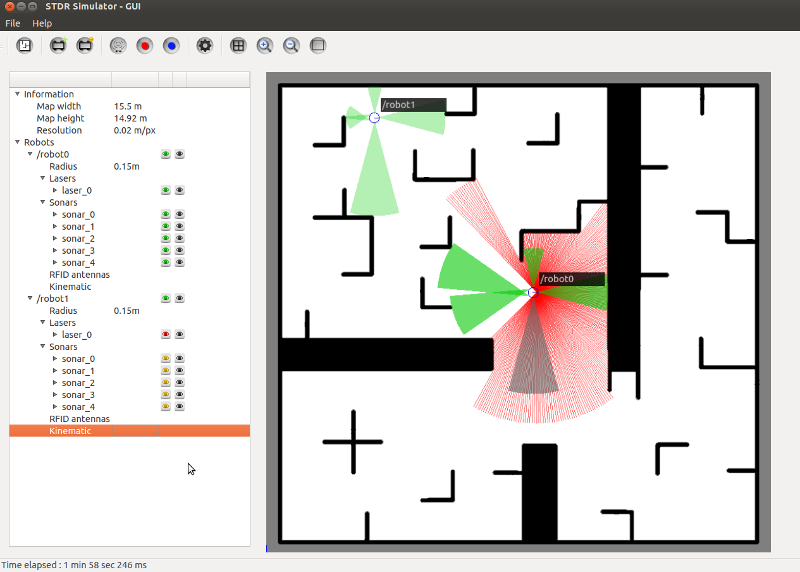
\includegraphics[width=0.75\textwidth]{./Images/Sprint0_STDR}
	\end{center}
	\caption{The original STDR 2D robot simulator, which the client initially wanted the team to modify.  \label{stdr}}
\end{figure}

\subsection{Clickable UI}

The clickable UI prototype consisted of buttons and slots partitioned into three sections: Simulation Mode, Map Mode, and Robot Mode. The intention during production of this prototype was to emulate a video game designer and produce a visual deliverable for the client. A blank black widget is visible where the world view is supposed to be, as this prototype did not have the world view integrated into the UI.\newline\newline\newline
\newline\newline\newline
\newline\newline\newline

\begin{figure}[H]
	\begin{center}
		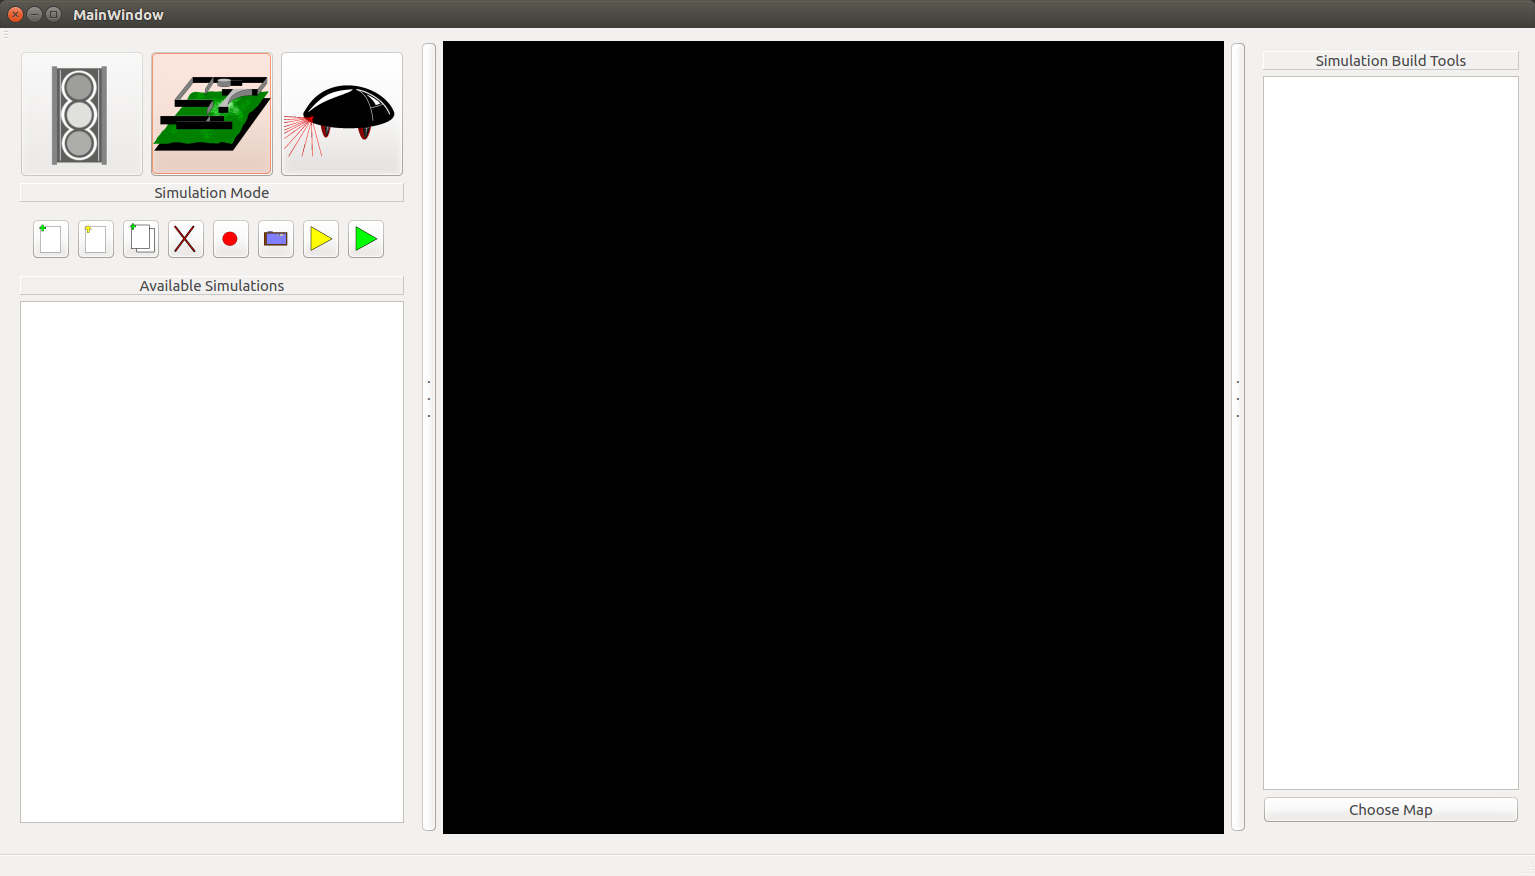
\includegraphics[width=0.60\textwidth]{./Images/Sprint1_clickableUI_SimulationMode}
	\end{center}
	\caption{The clickable UI with Simulation Mode, currently set in Simulation Mode.  \label{clickableuisimulation}}
\end{figure}

\begin{figure}[H]
	\begin{center}
		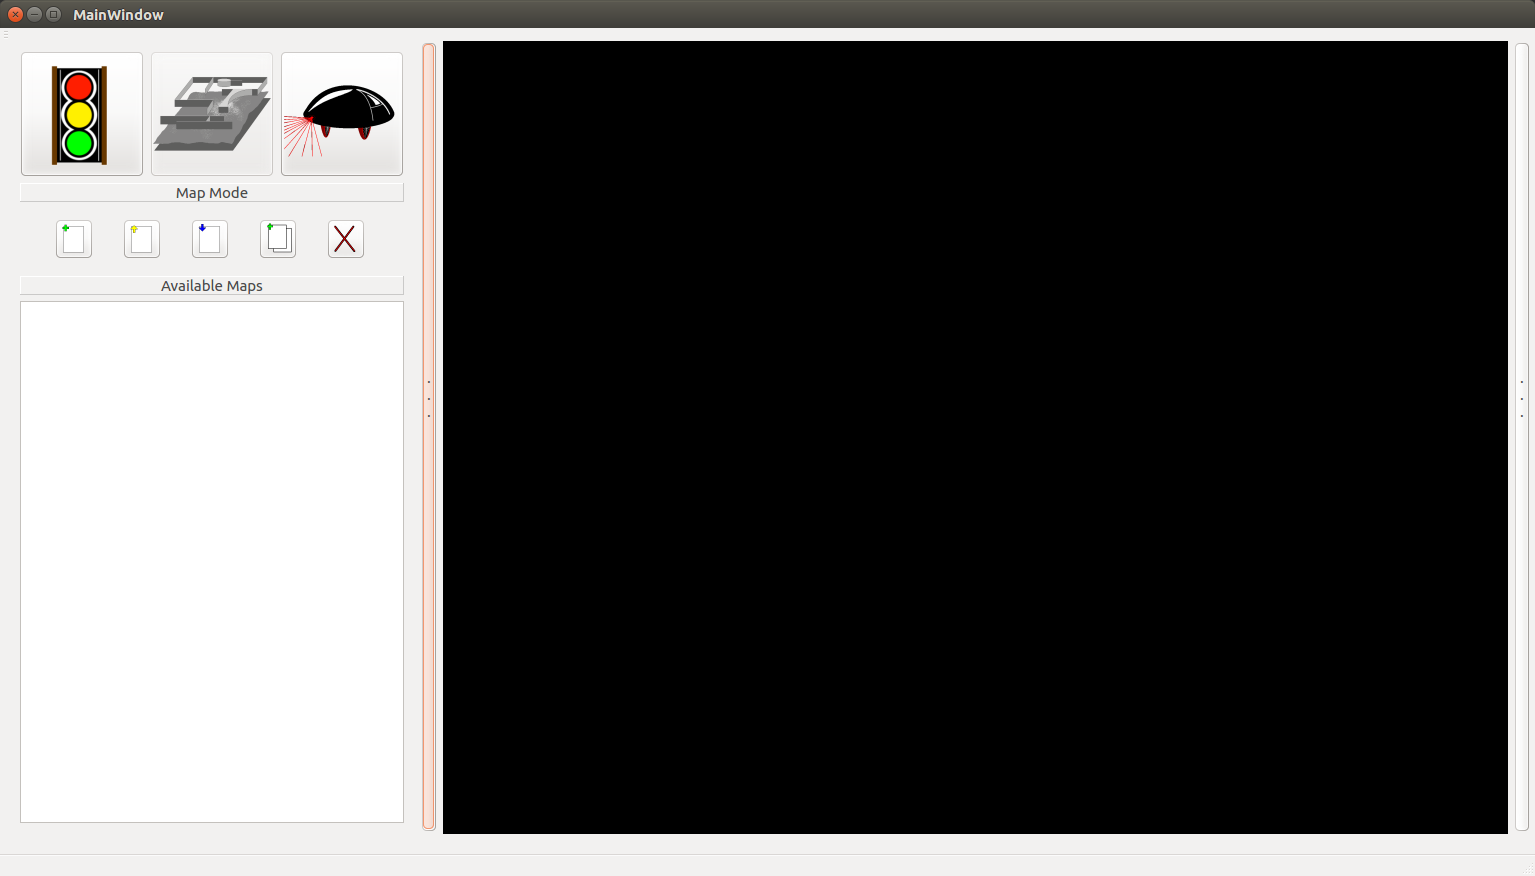
\includegraphics[width=0.60\textwidth]{./Images/Sprint1_clickableUI_MapMode}
	\end{center}
	\caption{The clickable UI, currently set in Map Mode. \label{clickableuimap}}
\end{figure}

\begin{figure}[H]
	\begin{center}
		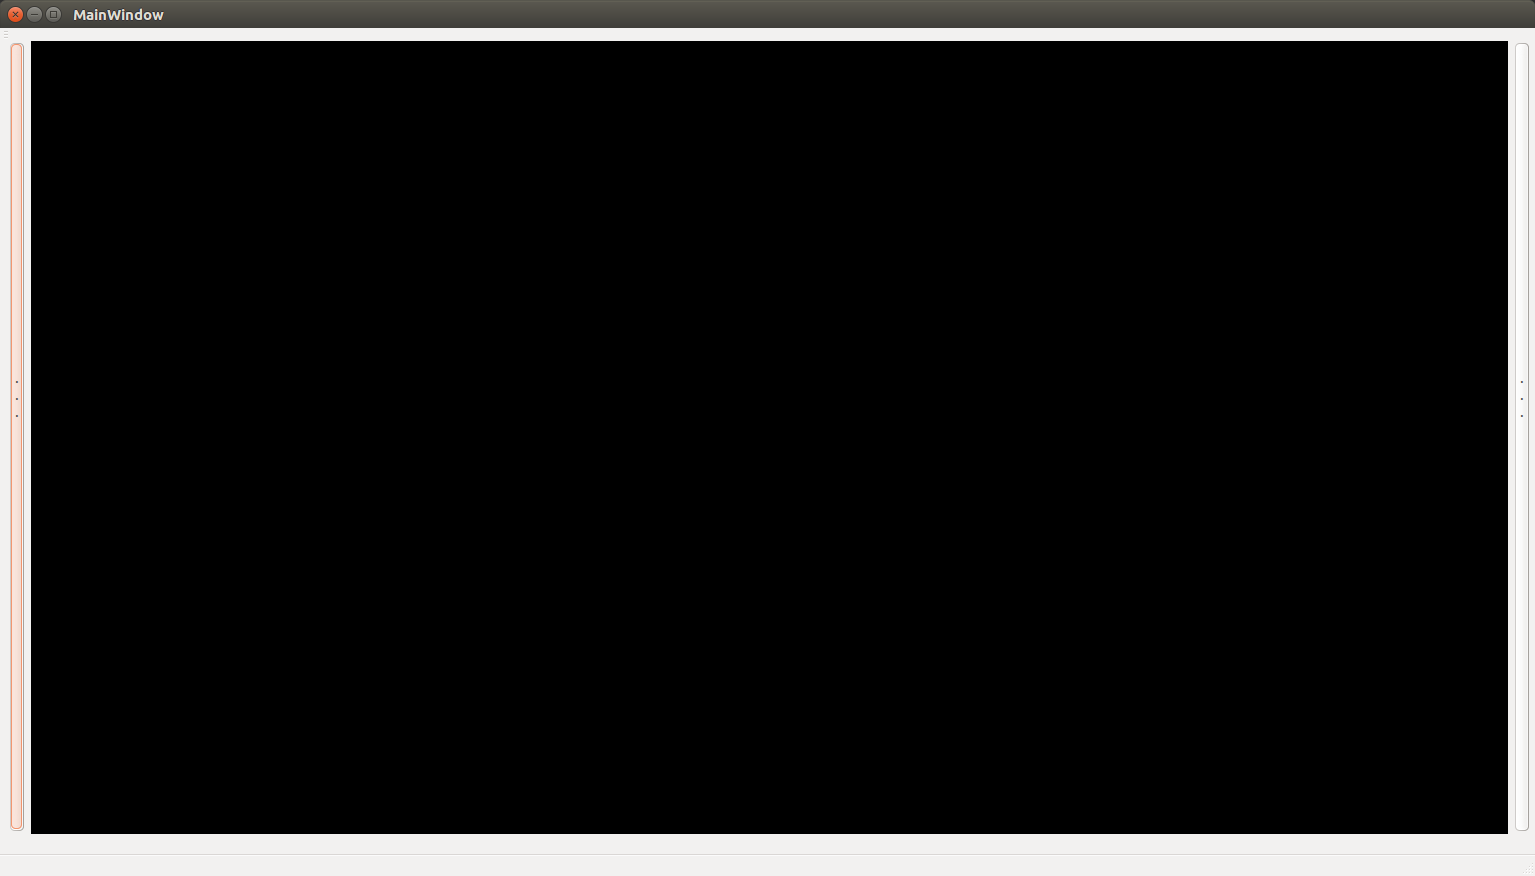
\includegraphics[width=0.60\textwidth]{./Images/Sprint1_clickableUI_NoMenus}
	\end{center}
	\caption{The clickable UI with side menus "minimized", a design decision based on the possible need to view robots moving on a larger map more easily. \label{clickableuinomenus}}
\end{figure}

\subsection{Modified MVP}

The original MVP consisted of a single robot spawning in the center of the world view and moving in a figure-8 with no obstacles to collide with. Here is the modified MVP from sprint four, in which three robots get spawned randomly throughout the world view. Also pictured is the "room" made up of four map objects which are static squares loaded from an obstacle file. Properties for one of the robots are listed on the menu to the left.

\begin{figure}[!htb]
	\begin{center}
		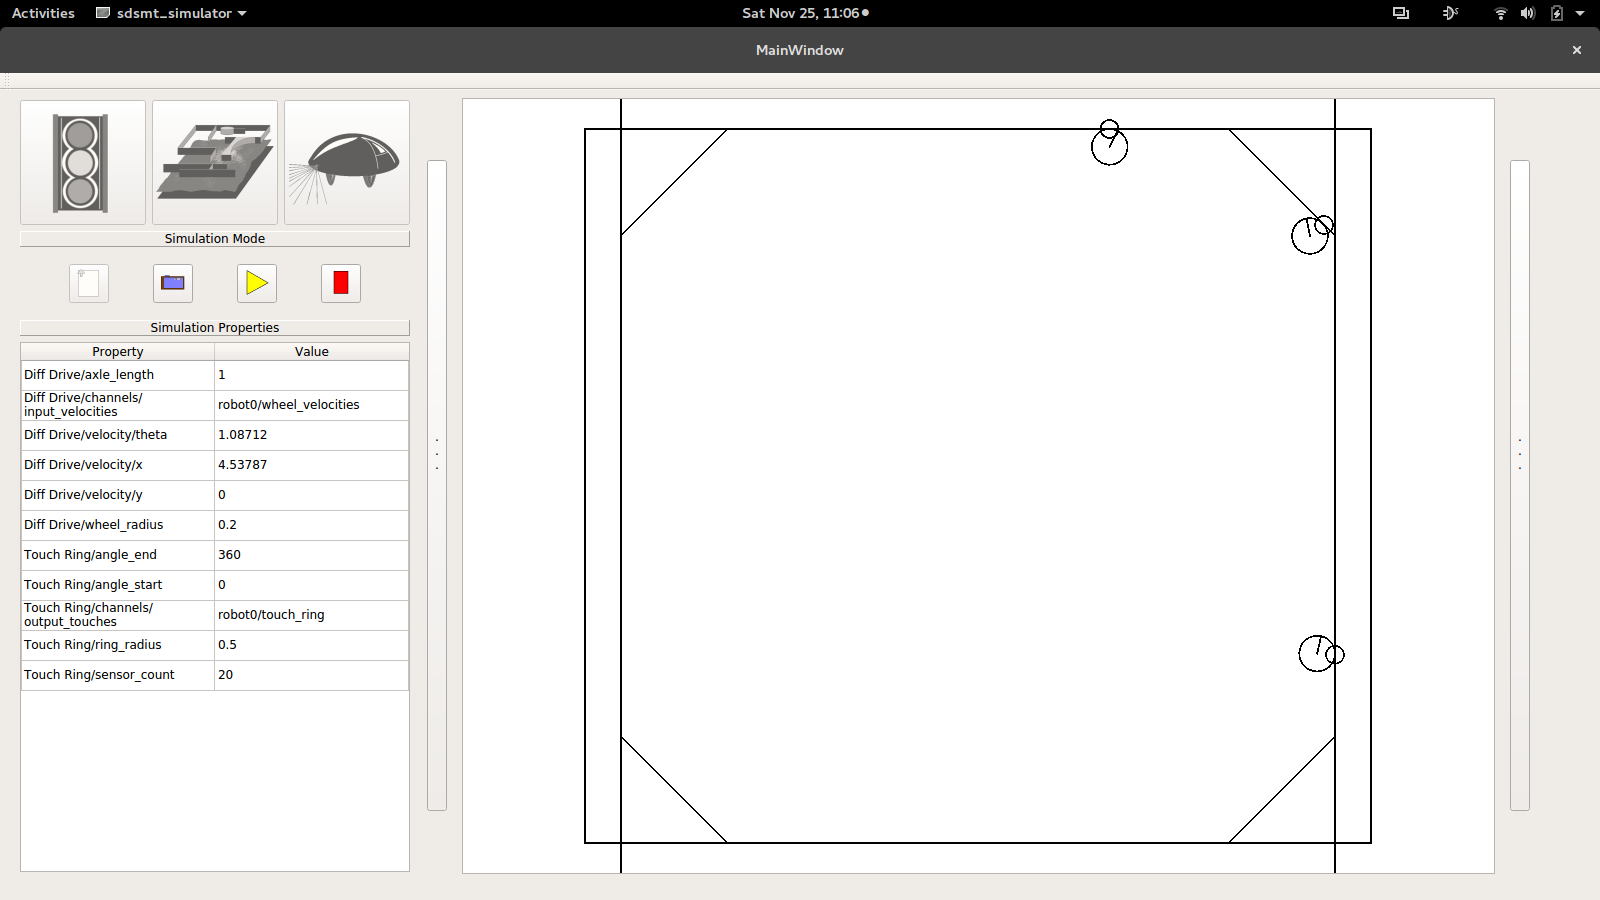
\includegraphics[width=0.75\textwidth]{./Images/Sprint3_hasBox_originalUI}
	\end{center}
	\caption{The MVP of our product, with a loaded map of four squares and three differential drive robots spawned at random locations in various orientations in the world view. \label{mvp}}
\end{figure}  %% All tracks
% !TEX encoding = UTF-8 Unicode
% !TEX root = DesignDocument.tex

\chapter{Release -- Setup -- Deployment}
This section should contain any specific subsection regarding specifics in releasing, 
setup, and/or deployment of the system. 


\section{Deployment Information and Dependencies}
Are there dependencies that are not embedded into the system install? 



\section{Setup Information}
How is a setup/install built? 



\section{System  Versioning Information}
How is the system versioned? 
  %% Normally not research track

\IfFileExists{UserMan/userManual.pdf}{
    \chapter{User Manual}
    \includepdf[pages=-]{UserMan/userManual.pdf}  %% All tracks
}{}

\bibliographystyle{plain}
\bibliography{designrefs.bib}
\addcontentsline{toc}{chapter}{Bibliography}


% We want to add the Software agreement to the end and number the
% pages separately from the document.  We don't want to do a standard
% chapter heading, but we do want it to appear in the table of contents
% and in the index used for on-line viewing.  We defined the \agreement
% macro to set things up for us.
\agreement

\IfFileExists{../Contract/contract.pdf}{
    \chapter{Software Agreement}
    \includepdf[pages=-]{../Contract/contract.pdf}
}{}

% In our style file, appendices are numbered with capital letters
\appendix

%\chapter{Product Description}
%
Write a description of the product to be developed.
Use sectioning commands as neccessary.
\vspace{2\baselineskip}

\centerline{\Large {\bf NOTE:} {\em This is part of the contract.}}



\IfFileExists{../Latex-Reference/refman.pdf}{
    \chapter{Software Documentation (Generated by Doxygen)}
    \includepdf[pages=-]{../Latex-Reference/refman.pdf}  %% All tracks
}{}

%\chapter{Acknowledgment}
%\label{SpecialThanks}  
%Thanks  

%\chapter{Supporting Materials}
%
This document will contain several appendices used as a way to separate out major 
component details, logic details, or tables of information.  Use of this structure 
will help keep the document clean, readable, and organized. 



\end{document}
